\documentclass{tudelft-report}
\usepackage{geometry}
\usepackage{hyperref}
\usepackage[noabbrev]{cleveref}
\usepackage{todonotes}
\presetkeys{todonotes}{inline, noline}{}
\usepackage{caption}
\usepackage{subcaption}
\usepackage{enumitem}
\usepackage{listings}
\graphicspath{{img/}}

% Source code listing style.
\lstset{%
  breaklines=true,
  captionpos=b,
  frame=none,
  keepspaces=true,
  numberstyle=\ttfamily
}

% Table markup:
% 1. Rotate column heads.
% 2. Define check- and crossmarks.
% 3. Top and bottom rules.
\newcommand*\rot{\rotatebox{-50}}
\usepackage{pifont}
\newcommand{\cmark}{\ding{51}}
\newcommand{\xmark}{\ding{55}}
\usepackage{booktabs}

\title{Generating REPLs for Spoofax}
\subtitle{Initial Research Report}
\author{%
Gerlof Fokkema\\
Jente Hidskes\\
Skip Lentz}
\date{\today}
\affiliation{Technische Universiteit Delft}

% Set cover image here.
%\coverimage{cover-filename}
\setpagecolor{tudelft-black}
%%% Local Variables:
%%% mode: latex
%%% TeX-master: "main"
%%% End:


\lstdefinelanguage{nabl}{
  % list of keywords
  morekeywords={
    namespaces,
    binding, rules,
    imports,
    from,
    implicitly, defines,
    of, type,
    scopes
  },
  sensitive=false, % keywords are not case-sensitive
  morecomment=[l]{//}, % l is for line comment
  morecomment=[s]{/*}{*/}, % s is for start and end delimiter
  morestring=[b]" % defines that strings are enclosed in double quotes
}
\lstdefinelanguage{type-spec}{
  % list of keywords
  morekeywords={
    type, rules,
    where, store, definition, of,
    and, else, on, error
  },
  otherkeywords={@},
  sensitive=false, % keywords are not case-sensitive
  morecomment=[l]{//}, % l is for line comment
  morecomment=[s]{/*}{*/}, % s is for start and end delimiter
  morestring=[b]" % defines that strings are enclosed in double quotes
}
\lstdefinelanguage{stratego}{
  % list of keywords
  morekeywords={
    rules, strategies
  },
  otherkeywords={
    <+, ->, ;, |, \[, \]
  },
  sensitive=false, % keywords are not case-sensitive
  morecomment=[l]{//}, % l is for line comment
  morecomment=[s]{/*}{*/}, % s is for start and end delimiter
  morestring=[b]" % defines that strings are enclosed in double quotes
}
\lstdefinelanguage{dynsem}{
  % list of keywords
  morekeywords={
    rules,
    where
  },
  otherkeywords={
    |-, -->
  },
  sensitive=false, % keywords are not case-sensitive
  morecomment=[l]{//}, % l is for line comment
  morecomment=[s]{/*}{*/}, % s is for start and end delimiter
  morestring=[b]" % defines that strings are enclosed in double quotes
}

\begin{document}

\frontmatter

\makecover

\begin{titlepage}
  \begin{center}
    %% Print the title.
    {\makeatletter
    \largetitlestyle\fontsize{64}{94}\selectfont\@title
    \makeatother}

    %% Print the optional subtitle in black.
    {\makeatletter
    \ifx\@subtitle\undefined\else
        \bigskip
       {\tudsffamily\fontsize{22}{32}\selectfont\@subtitle}
    \fi
    \makeatother}

    \bigskip
    \bigskip

    by

    \bigskip
    \bigskip

    {\makeatletter
    \largetitlestyle\fontsize{26}{26}\selectfont\@author
    \makeatother}

    \bigskip
    \bigskip
    \vfill

    {\makeatletter\large
    Compiled with \XeLaTeX\ on \@date\par
    \makeatother}

    \bigskip
    \bigskip
    \vfill

    \begin{tabular}{lll}
      Authors:             & Gerlof Fokkema             & 4257286 \\
                           & Jente Hidskes              & 4335732 \\
                           & Skip Lentz                 & 4334051 \\
      Client:              & Prof.~dr.~Eelco~Visser,    & Technische Universiteit Delft \\
      Coach:               & Hendrik van Antwerpen,     & Technische Universiteit Delft
    \end{tabular}

    \vfill
    \includegraphics[trim=0 5mm 0 0, width=40mm]{TU_Delft_logo_Black.eps}
  \end{center}
\end{titlepage}
%%% Local Variables:
%%% mode: latex
%%% TeX-master: main
%%% End:


\chapter{Preface and Acknowledgements}
\label{cha:preface-acks}

This report comprises the end of the TU Delft Computer Science Bachelor Project;
the final, compulsory project at the Delft University of Technology to attain
the Bachelor of Science in Computer Science.

The client during this project was the SLDE group at the TU Delft, who
\textit{``conduct research into concepts and techniques for programming language
design and implementation. The flagship product of the group is the Spoofax
Language Workbench''}. The Spoofax Language Workbench was to be extended with a
Read-Eval-Print Loop that would allow language designers and -users to
interactively work with the domain specific languages generated with Spoofax.

The purpose of this report is to describe the project as it was carried out over
the course of ten weeks. Not only does it describe the process, it also aims to
inform the reader about the problem and the design and implementation of the
solution to this problem. Finally, recommendations are made to the client to
improve the delivered product.

\section*{Acknowledgements}

We would like to thank Eelco Visser for the project proposal and the
opportunity to do our project under his supervision, Hendrik van Antwerpen for
being an excellent coach, Vlad Vergu for his collaboration and assistance with
DynSem and Gabri\"el Konat for answering several of our questions.

%%% Local Variables:
%%% mode: latex
%%% TeX-master: "main"
%%% End:


\chapter{Summary}
\label{cha:summary}

\textit{``The Spoofax Language Workbench supports the definition of all aspects
of textual languages using high-level, declarative meta-languages. From a
language definition using these meta-languages, Spoofax generates full-featured
Eclipse and IntelliJ editor plugins, as well as a command-line interface.''}

A feature that Spoofax is lacking is a Read-Eval-Print Loop (REPL) service. A
REPL is an interactive programming environment that takes single expressions,
evaluates them and prints the result(s). REPLs facilitate exploratory
programming and debugging and are therefore a nice addition to Spoofax.

This report comprises the end of the TU Delft Computer Science Bachelor Project;
the final, compulsory project at the Delft University of Technology to attain
the Bachelor of Science in Computer Science.

The purpose of this report is to describe the project as it was carried out over
the course of ten weeks. Not only does it describe the process, it also aims to
inform the reader about the problem and the design and implementation of the
solution to this problem. Finally, recommendations are made to the client to
improve the delivered product.

%%% Local Variables:
%%% mode: latex
%%% TeX-master: "main"
%%% End:


\tableofcontents{}

\mainmatter

\chapter{Introduction}
\label{cha:introduction}

General purpose programming languages such as Java and C have historically been
the most prevalent in the field of computer science. Nowadays a wide variety of
domain specific languages is also available, each of which is designed to
efficiently solve particular domain specific issues. \textit{``Domain-specific
languages (DSLs) provide high expressive power focused on a particular problem
domain. They provide linguistic abstractions and specialized syntax
specifically designed for a domain, allowing developers to avoid boilerplate
code and low-level implementation details''}~\cite{Kats10a}. Well known
examples of such DSLs include HTML for creating websites and SQL for dealing
with relational data.

At the Delft University of Technology, the Software Language Design and
Engineering group researches and develops domain specific languages. To
facilitate prototyping and creation of DSLs, the Spoofax Language Workbench was
developed and first published in 2010~\cite{Kats10a}. Since then Spoofax has had
several releases and will soon be arriving at version number 2.0. The
description below is taken from \href{http://spoofax.org}{the Spoofax website}:
\textit{``The Spoofax Language Workbench supports the definition of all aspects
of textual languages using high-level, declarative meta-languages. From a
language definition using these meta-languages, Spoofax generates full-featured
Eclipse and IntelliJ editor plugins, as well as a command-line interface.''}

A feature that Spoofax is lacking is a Read-Eval-Print Loop (REPL) service. A
REPL is an interactive programming environment that takes single expressions,
evaluates them and prints the result(s). REPLs facilitate exploratory
programming and debugging and are therefore a nice addition to Spoofax.

This report details how such a REPL has been implemented over the course of the
TU Delft Computer Science Bachelor Project. First of all an overview of the
required background needed to understand the problem domain is given in
\cref{cha:background}. In \cref{cha:probl-defin-analys} the problem definition
is then framed in the context of this background. The design and implementation
of the final product are discussed in \cref{cha:design} and
\cref{cha:implementation}. After this \cref{cha:evaluation} evaluates both the
final product and the process leading up the final product. The whole
project is reflected upon in the discussion in \cref{cha:discussion}, after
which recommendations regarding the final product are made in
\cref{cha:recommendations}. \Cref{cha:conclusion} then concludes this report.

%%% Local Variables:
%%% mode: latex
%%% TeX-master: "main"
%%% End:


\chapter{Background}
\label{cha:background}

This chapter gives the required background information required to
understand the rest of this report. If the reader is already well-versed in
Spoofax and familiar with a REPL, this chapter can be skipped.

The first section, \cref{sec:spoofax}, briefly explains what Spoofax is and what
services it provides to the language designer. \Cref{sec:repl} gives a quick
overview of what a REPL is and what advantages it offers to programmers.

\section{The Spoofax Language Workbench}
\label{sec:spoofax}
Spoofax is a platform that allows for giving a completely \emph{declarative}
definition of a programming language and accompanying IDE
support~\cite{Kats10a}. Such a platform is called a \emph{language workbench}.

In discussing programming languages, it is useful to distinguish the following
three concepts: an \textit{aspect} of a language, the formal
\textit{specification} of that aspect, and the actual \textit{implementation} of
that aspect, which follows from the specification. Any programming language can
be divided into multiple distinct aspects. In \cref{fig:spoofax-relations}, four
common aspects of programming languages are shown, along with the relation
between the formal specification and implementation for each aspect. An example
of an aspect is the \textit{syntax definition}: its formal specification is done
with grammar rules, and its implementation consists of both a tokenizer and
parser.

A key property of Spoofax is that it allows a language designer to give a
complete specification of each aspect of their language, and automatically
derive the implementation of that language aspect from its
specification. Spoofax provides a range of high-level, declarative
\textit{meta-languages} to the language designer for declaring their language
specification.

This section goes over the aspects that come into play with the development of a
language and how Spoofax tackles each of these aspects with its
meta-languages. First, the section goes over some of the elements that make up
the specification of each language aspect\footnote{This section follows the
  structure of the language specification portion of the compiler construction
  course at the TU Delft. The slides can be found here:
  \url{http://tudelft-in4303.github.io/lectures/specification/}.}. A language
commonly consists of the following aspects, shown also in
\cref{fig:spoofax-relations}, of which a selection will be discussed in more
detail throughout the rest of this section:

\begin{enumerate}
\item \textbf{\hyperref[ssec:syntax-def]{Syntax Definition}:} The first aspect
  concerns what textual representations of a program are syntactically
  valid. Its specification consists of a grammar specified with context-free
  grammar productions. A parser provides an implementation of this
  specification, by mapping a textual representation of a program to an abstract
  syntax tree (AST) representation. In Spoofax, the syntax is declared with a
  domain specific language (DSL) called SDF.
\item \textbf{Static Semantics:} A parsed AST then optionally goes through
  static analysis (type checking, name binding and variable scoping), to test if
  the program is well-formed. Static analysis is the implementation of an aspect
  called \textit{static semantics}. The static semantics of a language can be
  formally specified by \textit{type and/or name binding rules}. Spoofax
  provides two DSLs that can specify the two distinct parts of the
  specification: the TS Type Specification language and the NaBL name binding
  language.

  This language aspect will not be discussed in this section. However, the
  original research report contains a section that does discuss this aspect, and
  can be found in \cref{ssec:a-static-analysis}.
\item \textbf{Term Rewriting or Program Transformation:} Optionally, a
  well-formed AST can then be transformed, for example for desugaring or
  optimization. This execution step falls under the aspect of \textit{term
    rewriting} and can be formally specified by \textit{term rewrite rules}. For
  the specification of this aspect, Spoofax provides a DSL called Stratego.

  This aspect, too, will not be discussed in this section. The relevant section
  in the research report can be found in \cref{ssec:a-term-rewrite}.
\item \textbf{\hyperref[ssec:dynamic-semantics]{Dynamic Semantics}:} Next the
  optionally transformed AST is either compiled or interpreted, thereby
  providing a means of execution. The aspect of \textit{dynamic semantics}
  defines what the behaviour is of a program upon execution. The formal
  specification of this aspect can be done with \textit{reduction rules},
  although there are other ways to accomplish this: for example, interpretation
  can be seen as the transformation of a program to a single value. In Spoofax,
  the dynamic semantics can be defined with either Stratego or a DSL called
  DynSem.
\end{enumerate}

\begin{figure}[t]
  \centering
  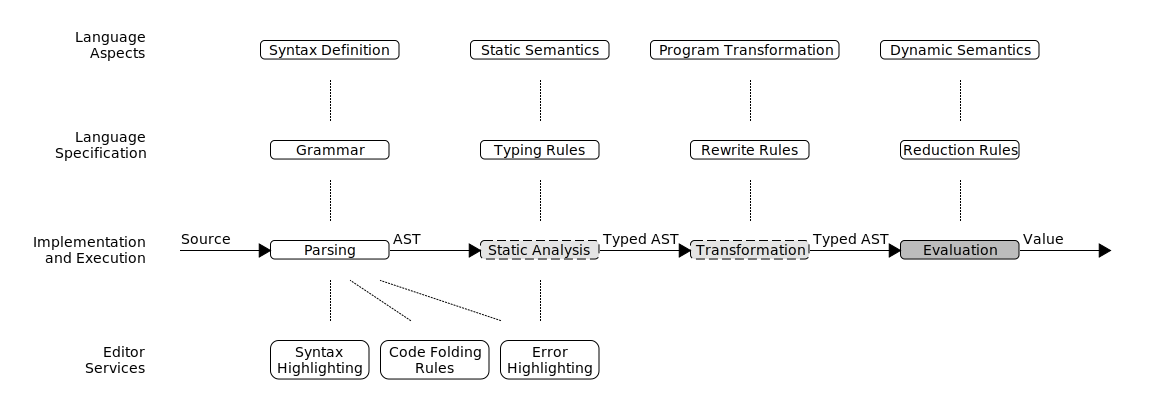
\includegraphics[width=\textwidth]{spoofax-relations}
  \caption{The relations between the aspects, specification and implementation
    of a programming language. The dashed boxes in the bottom row refer to that
    step being optional.}
  \label{fig:spoofax-relations}
\end{figure}

This section concludes with a discussion on the other part of a language: its
integrated development environment (IDE). Spoofax provides IDE support by means
of its Editor Services.

\subsection{Syntax Definition}
\label{ssec:syntax-def}
The first part of the specification of a language is its syntax. The
syntax of a language is often specified by means of a \emph{lexical
grammar} and a \emph{context-free grammar}, as can be seen in the
specification of, for example, Standard ML~\cite{Milner97}. The
lexical grammar is most often defined using regular expressions. It
defines the individual words made up of characters, such as
identifiers and numeric constants. The context-free grammar then
defines syntactically valid sentences made up of words.

\subsubsection{SDF3: syntax definition in Spoofax}
\label{ssec:orgheadline1}
To specify a syntax definition declaratively in Spoofax, a DSL called
\emph{SDF3}~\cite{Vollebregt12} is used.  SDF3 is the third generation
of the \emph{Syntax Definition Formalism} (SDF)~\cite{Heering89}. It
uses only context-free grammer productions for the specification of
both the lexical syntax and the context-free syntax, a feature that
was introduced in SDF2~\cite{Visser97}.

The declarative nature of SDF3 allows for thinking in terms of the
structure (the \emph{what}), instead of in terms of parser algorithms (the
\emph{how}) as is the case with many current parser generators such as
ANTLR and YACC~\cite{Kats10b}. The syntax definition is used to
make parsers that parse a textual representation of a program into its
AST and pretty-printers for mapping ASTs back to text. However, due to
its declarative nature, SDF3 is not limited to generating parsers and
pretty printers: it can also be used for error recovery
rules~\cite{deJonge12}, syntax highlighting rules and folding
rules for editors (see \cref{ssec:editor-serv}).

The Spoofax API gives access to the generated parser through the
\texttt{SyntaxService}.

\subsubsection{ASTs in Spoofax: Stratego Terms}
\label{sec:asts-spoof-strat}
% TODO: Reference for Stratego terms.
In Spoofax, an AST is represented as a Stratego term, a format representing tree
structures that comes with a textual representation similar to formats such as
XML. As an example, a representation of the arithmetic expression $2 + 2 - 4$ is
shown in \cref{lst:aterm-example}.

\begin{lstlisting}[caption={An example Stratego term representation of an
arithmetic expression},language=aterm,label={lst:aterm-example}]
Sub(Add(Int("2"), Int("2")), Int("4"))
\end{lstlisting}

Stratego terms can however represent any tree structure, not just ASTs. As such,
when using Spoofax programmatically through its API, one sees Stratego terms
used as an internal representation of the data going through the execution
pipeline depicted in \cref{fig:spoofax-relations}.

\subsection{Dynamic Semantics}
\label{ssec:dynamic-semantics}
Dynamic semantics refers to how a program written in some language
behaves~\cite{Winskel93}. There are many approaches to formally specify the
dynamic semantics of a programming language (for an extensive treatment,
see~\cite{Winskel93}). One way is to specify the transformation of programs
written in the programming language to programs of another language of which the
dynamic semantics are already known. For this report, however, only one sort
of approach called \emph{operational semantics} is relevant.

The first part of this subsection gives a short description of operational
semantics, and shows an example of how it can be used to specify the dynamic
semantics of a programming language. After that, a short overview of DynSem is
given, as well as the same example expressed in DynSem.

\subsubsection{Operational semantics}
\label{sec:oper-semant}
In operational semantics, the dynamic semantics are specified by a set of axioms
and reduction rules. A reduction rule consists of set of premises and a
predicate. If all of the premises of a reduction rule hold, then the predicate
also holds~\cite{Kahn87}. A predicate is structured as follows: the left-hand
side of a formula introduces a pattern, and the right-hand side instantiates the
result.

To show how rules can define the dynamic semantics of a language, consider the
classic example of the \(\beta\)-rule shown in \cref{eq:beta-reduct-structural},
which defines function application in the lambda calculus. The rule replaces all
the occurrences of the parameter \(x\) with the argument \(e_2\), within the
expression \(e_1\).

\begin{equation}\label{eq:beta-reduct-structural}
(\lambda x.e_1) e_2 \xrightarrow{\beta} e_1[x := e_2]
\end{equation}

\begin{equation*}\label{eq:beta-reduct-natural}
\infer{%
  E \vdash e_1 e_2 \rightarrow v%
  }{%
    \begin{split}
      E \vdash e_1 \rightarrow (\lambda x.b, E') \\
      (x \mapsto e_2) \circ E' \vdash b \rightarrow v
    \end{split}%
}
\end{equation*}

\subsubsection{DynSem: rule-based dynamic semantics}
\label{ssec:dynsem}
Aside from Stratego, the Spoofax team has developed an additional
method to declare the dynamic semantics of a language, namely a DSL
called \emph{DynSem}~\cite{VerguNV15}. DynSem allows for an operational
semantics specification from which a Java-based AST interpreter is
automatically generated.

\paragraph{Reduction rules} In DynSem, reduction rules are used to specify the
dynamic semantics of a language, in a syntax similar to the formal syntax like
shown in \cref{eq:beta-reduct-natural}. A reduction rule in DynSem takes the
following form~\cite{VerguNV15}:

\begin{minipage}[t]{\linewidth}
\begin{lstlisting}[language=dynsem,numbers=left,caption={The syntactic structure
of a reduction rule in DynSem.},label={lst:dynsem-rule-syntax}]
  Rs |- <term1> :: RWs --> <term2> :: RWs'
  where <premise1>;
        <premise2>.
\end{lstlisting}
\end{minipage}

The rule as shown in \cref{lst:dynsem-rule-syntax} is read as follows: given
that the conditions \texttt{premise1} and \texttt{premise2} can be satisfied,
perform a pattern-match on \texttt{term1} and instantiate the pattern
\texttt{term2} as the result of the reduction.

\paragraph{Semantic components} The variables \texttt{Rs}, \texttt{RWs} and
\texttt{RWs'} shown in \cref{lst:dynsem-rule-syntax} are called \textit{semantic
  components}: they represent the context in which the reduction takes place. An
example of a semantic component is that of an environment, which maps variable
names to their values. Another example is that of a store, which maps addresses
of values to the values themselves. There are two kinds of semantic components:
\textit{read-only} semantic components and \textit{read-write} semantic
components. An environment is a read-only semantic component: a variable is
bound only within a certain scope, and any other reduction rules that are
applied outside of that scope don't see this environment. A store is a
read-write semantic component: changes in the store are visible everywhere, as
it represents mutable state.

\paragraph{Function application in DynSem} Two examples of reduction rules are
shown in \cref{lst:dynsem}. Taken together the rules specify the semantics of
function application by using an environment, rather than replacement as done in
\cref{eq:beta-reduct-structural}:

\begin{minipage}[t]{\linewidth}
\begin{lstlisting}[language=dynsem,numbers=left,caption={Specifying function
application through the use of an environment.},label={lst:dynsem}]
rules
  E |- Fun(x, e) --> ClosV(x, e, E).

  App(ClosV(x, e, E), v1) --> v2
  where
    E  |- bindVar(x, v1) --> E';
    E' |- e --> v2.
\end{lstlisting}
\end{minipage}

The first rule, shown in line 2, captures the notion of a closure, which is
merely a function together with the environment it is defined in. The
environment variable \texttt{E} is matched on the left-hand side, and used in
the result of the rule on the right-hand side.

The second rule, corresponding to lines 4 to 7, first introduces a pattern-match
on a term representing function application. In line 6, the environment
\texttt{E} is extended with a variable binding \texttt{x -> v1} to form a new
environment \texttt{E'}. Then in line 7 the function body \texttt{e} is reduced
to the value \texttt{v2}, within the context of the newly extended environment
\texttt{E'}.

\subsection{Editor Services}
\label{ssec:editor-serv}
This section concludes with a brief description of editor services,
which provide the IDE support for languages defined in
Spoofax. Examples of such services include an outline view, menus in
which one can bind actions to menu buttons (see
\cref{fig:menu-actions}), but also syntax highlighting, syntactic code
completion and code folding rules\footnote{More services are
listed on the Spoofax website:
\url{http://www.metaborg.org/spoofax/editor-services/}}.

The Spoofax API provides the editor services with similar naming. For
example, the outline can be retrieved from the \texttt{OutlineService}, the
syntax highlighting can be accessed through the \texttt{StylerService} and
syntactic code completion is accessed with the
\texttt{CompletionService}. The defined menus for a particular language can
be retrieved with the \texttt{MenuService}, from which the menu actions can
be retrieved and used.

\begin{figure}[bt]
\centering
\includegraphics[width=0.6\textwidth]{./img/menu-actions.png}
\caption{\label{fig:menu-actions}
A menu action for the paplj language defined using Spoofax. The bottom window shows the menu definition, the top window shows a program written in paplj.}
\end{figure}

Editor services are defined using a DSL, shown in the bottom window of
\cref{fig:menu-actions}. In the case of menus, their actions are
specified using Stratego. Since Stratego supports native strategies,
these actions can also be specified in Java. As such, Spoofax allows
for defining arbitrarily complex IDE actions.

Many of these editor services such as syntax highlighting and code
folding rules can be derived from the syntax
definition~\cite{Kats10c} and can be further customized if
needed. Taken together with the language definition, the editor
services provide a language with a complete and state-of-the-art IDE
experience~\cite{Kats10a}.
%%% Local Variables:
%%% mode: latex
%%% TeX-master: "../main"
%%% End:


\section{Read-Eval-Print Loops}
\label{sec:repl}

Many programming languages come with an interactive environment. This
interactive environment is an interface to the programming language's execution
engine. One common form of such an environment is an interface in which
expressions in a programming language are typed by the user, after which the
results of that expression are printed back to the user. Such an environment is
called a Read-Eval-Print Loop (REPL), although many different names are known,
including but not limited to \emph{language shell}, \emph{command-line
  interpreter} or \emph{interactive interpreter}. In this report the term REPL
is chosen, because it conveys the notion of such an interactive environment
well.

\subsection{Origin of REPLs}
\label{ssec:repl-origin}

The Lisp programming language is one of the first programming languages offering
such an interactive environment~\cite{Noyes92}. The name REPL comes from the
Lisp functions that implement it:

\begin{enumerate}
  \item The \texttt{read} function takes a user's input, which often is just one
    or several expressions as opposed to a complete compilation unit. It then
    parses this input and creates an AST.
  \item The AST created in the previous step is then passed on to the
    \texttt{eval} function, which evaluates it.
  \item The result yielded by the previous function is then printed out to the
    user by the \texttt{print} function.
  \item After having printed the result, the environment needs to \texttt{loop}
    back to the read state.
\end{enumerate}

Assuming the individual functions listed previously exist, a REPL can be created
in a single line of code simply by combining the functions:

\begin{lstlisting}[language=lisp]
(loop (print (eval (read))))
\end{lstlisting}

Lisp has a property called ``homoiconicity'': Lisp's syntax is similar to
its internal representation, resulting in the ability to infer a program's or
data object's state simply by reading its textual representation. Syntax and AST
are thus isomorphic, allowing data and code to be accessed and transformed
interchangeably.

In Lisp REPLs, therefore, arbitrary data objects yielded from a previous
expression can be used directly as input to the next expression. In programming
languages that do not belong to the Lisp family, homoiconicity is an unusual
feature. Interactive environments for these languages therefore often require
additional steps to read and evaluate expressions. This is part of the semantic
differences between the different names as mentioned in the introduction

\subsection{Advantages of REPLs}
\label{ssec:repl-advantages}

REPLs provide the ability to program interactively. Programming interactively
has multiple advantages.

When creating software solutions for an as of yet not well understood domain, it
is often not clear which data structures and algorithms are required. In such
cases, interactively developing and debugging software is an advantage over the
(oftentimes much slower) edit-compile-run-debug development style. This kind of
programming is called exploratory programming~\cite{Fritzson86}. Related to this
kind of exploration, programming interactively also provides a means for rapid
prototyping and bottom up programming~\cite{Graham93}.

The explorative and interactive features of a REPL also make it an excellent
tool for programmers to learn a new programming language. REPLs are also
combined with what is called literate programming to offer notebooks or language
playgrounds, as discussed in \cref{sec:literate-programming}.

\subsection{Execution model}
\label{ssec:execution-model}

Every programming language defines an execution model, which specifies how
programs written in that language are executed. Among others, it specifies what
an indivisible unit of work is (a \emph{compilation unit}) and in what order
these units are executed. The implementation of an execution model is a compiler
and/or an interpreter. The execution model of a REPL as shown in
\cref{fig:execution-model-repl} has a couple of differences with respect to that
of an interpreter or compiler.

One difference is what is considered an indivisible unit of work: a REPL might
accept singular expressions that a regular interpreter or compiler might
not. Usually the program is executed as a whole, without the need for smaller
blocks of execution. In contrast, when using a REPL, it might be desirable to be
able to execute only a single statement as one unit of execution. The AST output
of the parsing step, as shown in \cref{fig:execution-model-repl}, can therefore
be a smaller unit than an AST found in the ordinary execution model.

Another difference between a compiler or an interpreter and a REPL is that a
REPL needs to dynamically maintain an environment such that each new expression
can be analyzed and evaluated within the environment of previously executed
expressions. For every expression entered, it thus needs to apply the outlined
steps again and update the environment it maintains in memory with the new
results. This could result in a different order of evaluation than when for
example an interpreter executes a program as a whole.

\begin{figure}[t]
  \centering
  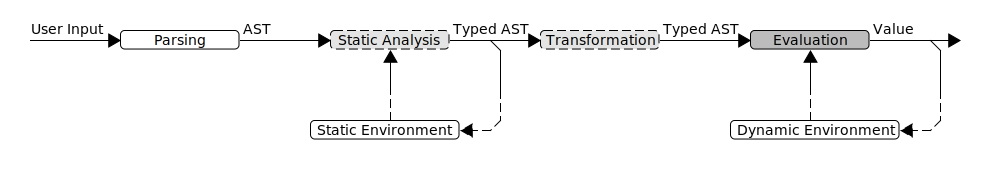
\includegraphics[width=\textwidth]{execution-model-repl}
  \caption{The execution model as shown in \cref{fig:spoofax-relations}, adapted
    for a REPL. The analysis and evaluation is done within the incrementally
    built environment of previously executed expressions.}
  \label{fig:execution-model-repl}
\end{figure}

\subsection{Functionality}
\label{ssec:repl-functionality}

Every REPL provided with a programming language has its own set of
functionality. However, a core set of functionalities, shared between all REPL
implementations, can be identified. To reach this core set of features,
well-known REPLs have been investigated and their features have been compiled
into a matrix as seen in \cref{table:feature-matrix}. These features are shortly
discussed below.

\begin{table}[]
\centering
\begin{tabular}{lccccccccc}
                                  & \rot{Python} & \rot{R} & \rot{\shortstack[c]{Common\\Lisp}} & \rot{\shortstack[c]{Haskell\\(GHCi)}} & \rot{Swift} \\
\toprule
Execution in context              & \cmark       & \cmark  & \cmark                             & \cmark                                & \cmark      \\
Input history                     & \cmark       & \cmark  & \cmark                             & \cmark                                & \cmark      \\
Automatic binding of previously yielded values & \xmark & \xmark & N/A                          & \xmark                                & \cmark      \\
Persistent input history          & \cmark       & \cmark  & \xmark                             & \cmark                                & \cmark      \\
Multiline input editing           & \cmark       & \cmark  & \cmark                             & \cmark                                & \cmark      \\
Redefining identifiers            & \cmark       & \cmark  & N/A                                & \cmark                                & \cmark      \\
Error reporting                   & \cmark       & \cmark  & \cmark                             & \cmark                                & \cmark      \\
Semantic code completion          & \cmark       & \xmark  & N/A                                & \xmark                                & \cmark      \\
Help or documentation system      & \cmark       & \cmark  & \cmark                             & \xmark                                & \xmark      \\
Additional commands to the REPL   & \xmark       & \xmark  & \cmark                             & \cmark                                & \cmark      \\
Nested REPLs to enable debugging  & \xmark       & \xmark  & \cmark                             & \xmark                                & \xmark      \\
\bottomrule
\end{tabular}
\caption{A feature comparison of several well-known REPLs}
\label{table:feature-matrix}
\end{table}

\paragraph{Execution in context} Expressions that are entered are executed
within the context of previous executions.

\paragraph{Input history} REPLs keep a history of inputs, such that previously
entered expressions can be retrieved.

\paragraph{Automatic binding of previously yielded values} When an expression
has been evaluated, the yielded result is bound to an automatically created
identifier, such that it can be reused easily in future expressions.

\paragraph{Persistent history} The input history as discussed previously can be
recorded into a file (either per-project or globally) to enable a persistent
history of input.

\paragraph{Multiline input editing} Some constructs in a programming language
naturally span multiple lines. REPLs therefore provide multiline input editors
that recognize incomplete code and promptly switch to a multiline environment
when required.

\paragraph{Redefining identifiers} When using a REPL in an exploratory manner,
it is not uncommon to want to redefine an identifier's type or to completely
reimplement a method. In this way, a REPL can be different than its host
language, especially if the host language is a functional language that does not
allow variables' values to change once initiated.

\paragraph{Error reporting} A REPL typically has the same error reporting
functionality as an interpreter or a compiler, meaning it prints the error
message accompanied by the corresponding section of the source code.

\paragraph{Semantic code completion} Semantic code completion is a helpful tool
to provide an overview of the often many APIs a developer works with, adding to
the explorative nature of a REPL. Note that this is a restriction of syntactic
completion, which is offered by all the studied REPLs.

\paragraph{Help or documentation system} The exploratory nature of a REPL means
that one will often see new methods. Some REPLs (most notably Python's REPL with
Python's docstrings) offer a documentation system, so that the developer does
not have to exit the REPL to look up documentation.

\paragraph{Additional commands to the REPL} Some REPLs offer additional commands
to inspect the environment or to control their behavior. These commands are
often not in the syntax of the host language and are highly diverse between REPL
implementations. A notable example of a REPL offering such commands is Haskell's
GHCi~\cite{GHCi-commands}.

\paragraph{Nested REPLs to enable debugging} A notable feature of (mostly) Lisp
REPLs is that in case of an error, a new REPL is spawned inside the context of
this error. This REPL then has additional commands (see the previous feature) to
enable debugging and inspection of the error state. When the user has
resolved the error, the nested REPL exits and the user is returned to the
parent REPL. This can go to arbitrary depths.

%%% Local Variables:
%%% mode: latex
%%% TeX-master: "../main"
%%% End:


%%% Local Variables:
%%% mode: latex
%%% TeX-master: "main"
%%% End:


\chapter{Problem Definition and Analysis}
\label{cha:probl-defin-analys}

\section{Problem Definition}
\label{sec:problem-definition}

In this section, the problem of the client is defined. First the
general problem is given in the form of a question. After that the
general definition will be divided into multiple sub-definitions.

Spoofax offers a wide variety of tools to develop DSLs and accompanying IDE
support. Precisely because Spoofax is concerned with developing DSLs, rapid
prototyping of syntax and grammar is a convenient addition to the product.
\Cref{sec:repl} showed that REPLs provide precisely this rapid prototyping
ability.  Therefore, the client has expressed their interest in a REPL that
works with languages designed with Spoofax. Such a REPL would aid both the
developer of the language and its end-user. The main problem, thus, can be
stated as a question as follows: \textit{``How can a REPL be created that can be
used with languages defined with Spoofax?''}.

Spoofax already provides a lot of language services that can be reused. However,
this is not without issues, as Spoofax's infrastructure currently is not geared
towards interactive use. A subquestion, then, is: \textit{``How can Spoofax's
services be changed to support both interactive and non-interactive use?''}.

% TODO: Java-backend example requires a cite?
Additionally, there are currently two ways to define the dynamic semantics of a
language (see \cref{ssec:dynamic-semantics}); one can either use DynSem or Stratego.
Some languages even define their own interpreter writtin in Java. Therefore,
another subquestion is: \textit{``How can the REPL support multiple
interpreters?''}.

As listed in \cref{ssec:repl-functionality}, REPLs provide many features. Some
of these are not yet available in Spoofax. These features are critical to
exposing the interactive exploration of programs in languages defined with
Spoofax. Examples include displaying and editing the contents of the current
program's context, saving and loading this context and keeping a history of
executed expressions. This forms the third subquestion: \textit{``How do these
additional features fit into Spoofax's existing architecture?''}.

When a REPL is realized in time, the product could be further extended to add
support for literate programming, allowing for rapid prototyping and
documentation at the same time~\cite{schulte2012}. This would allow
developers of new DSLs to document and explain their language in an
interactive manner that directly allows experimentation.

%%% Local Variables:
%%% mode: latex
%%% TeX-master: "../main"
%%% End:

\section{Problem Analysis}
\label{sec:problem-analysis}
This section section describes the problems that need to be solved while
incorporating a REPL within the larger context of Spoofax.

The general theme of the sub-problems that arise from the problem
defined in the previous section, is that the REPL should work
with any language defined with Spoofax. Languages differ in what
properties they have and how they are specified. For example, a
functional programming language with no mutability is specified
differently from an imperative and mutable programming
language. Finding a generic way to make the REPL work for all of these
languages, without any configuration from the part of the language
designer, is hard, and may even be impossible.

The solution to many of the problems is to identify which parts of the problem
can be solved generically, and which parts warrant configuration by the
language designer. When the REPL requires configuration by the language
designer, enough flexibility should be provided to do so with the least amount
of effort possible.

Each of \cref{ssec:supp-diff-ways,ssec:lang-spec-addit,ssec:repl-spec-semant}
discusses a more concrete instance of this general problem.

\subsection{Supporting different execution pipelines}
\label{ssec:supp-diff-ways}
Different Spoofax languages have different ways of executing a program.
For example, some languages have an analysis step, whereas
others do not. Moreover, specifying the dynamic semantics of a language
can be done in multiple ways (see \cref{ssec:dynamic-semantics}): one
can use DynSem, Stratego, and some languages even implement a Java
backend\footnote{See IceDust:
  \url{https://github.com/MetaBorgCube/IceDust}}.

Some of these properties of a language should be detected by the REPL
automatically, such as whether a language has an analysis step.
Other properties of a language, however, cannot be detected
automatically. For example, the REPL should be able to maintain an
execution environment for the duration of the REPL session, but
precisely what an execution environment looks like differs among
languages.

\subsection{Language-specific commands}
\label{ssec:lang-spec-addit}
Another problem is when some additional command can be useful for a
REPL of a particular language, but would not make any sense within the
context of other languages. For example, some languages such as Python
allow for loading modules, which brings all of the definitions inside
of these modules into scope. An additional command to load a module
could in that case be useful, but would not make any sense in
languages that have no concept of definitions that can be imported.

This problem could be solved by the language designer by extending
their language with reflective capabilities. However, the language
designer might not want to extend the language with reflective
capabilities outside of the context of a REPL. It is therefore clear
that a different approach should be considered.

\subsection{REPL-specific semantics}
\label{ssec:repl-spec-semant}
Sometimes a property of some language stands in the way of the rapid
prototyping capabilities that are desirable for a REPL. For example, a
language like Haskell does not allow for redefining a function's
implementation in its normal semantics, whereas in the context of a
REPL this is usually what one wants.

This poses a similar problem as in the previous section: adding REPL-specific
semantics to the language should not affect the original semantics of the
language. Therefore, requiring the language designer to change the original
semantics of the language is an inadequate solution.

%%% Local Variables:
%%% mode: latex
%%% TeX-master: "../main"
%%% End:

\section{Requirements Analysis}
\label{sec:requirement-analysis}

Defining requirements upfront is important for several reasons: it is a contract
between the developers and the client, it guides the product development, it
enables the client to track the progress and finally it allows for validation of the
deliverable. The requirements are listed in this section.

\subsection{Design goals}
\label{ssec:goals}

The client has expressed some high-level requirements, which are listed in this
section as design goals in order of priority. The design goals serve as an
important guideline when defining and implementing the invidual requirements. As
such, they can be considered the bounds within which all requirements must fit.

\paragraph{Language-agnostic} The REPL should not make any assumptions about its
host language: it must work with all languages defined with Spoofax. This also
means that a language-agnostic configuration interface must be provided, in
order to allow the language designer to configure and implement the
language-specific parts of the REPL. Note that this does not mean that the REPL
is expected to work out of the box for any language.

\paragraph{Minimal configuration} The REPL should require as little
configuration as possible. This means that the REPL allows the
language designer to reuse existing components of their language
definition in its configuration. Moreover, the language
designer should not have to configure areas of the REPL that can
instead be derived automatically.

\paragraph{Maintainability} Spoofax is an already existing, open source project
managed by several people. When the product is delivered, these people will take
over the maintainership. Therefore, it is important that the code is
maintainable. This means that the code should be well-documented, with low
coupling and high cohesion in the code's modules.

\paragraph{IDE-agnostic} Current stable releases of Spoofax integrate solely with
Eclipse. An effort is underway to make Spoofax IDE-agnostic and to
provide separate modules to tie Spoofax to IDEs. The REPL should keep this in
mind from the start and not tie itself to any IDE.

\paragraph{Performance} Spoofax's developers already focus quite a bit on
performance: both the generation and the use of the services are performant.
This should be no different for the REPL.

\paragraph{Modify Spoofax's existing codebase as little as possible} The product
should be an extension to Spoofax, which means the changes made to the existing
Spoofax codebase should be as small as possible. Preferably, the REPL service
should be a standalone module.

\subsection{Requirements}
\label{ssec:requirements}

Under the guidance of the design goals listed in the previous section, the
requirements compiled from the feature matrix discussed in \cref{sec:repl} and
meetings with the client are discussed below using the MoSCoW method.

\subsubsection{Must have}

Requirements listed under ``must have'' are of critical importance to the
usability and success of the deliverable. Without these, the product is not in a
workable state and is not likely to be accepted by the client. \emph{Must} can
also be considered an acronym for the Minimum Usable SubseT.

\paragraph{Interactive REPL} Per the definition of a REPL given in
\cref{sec:repl}, the REPL has to be interactive. It should evaluate single
statements and expressions typed in by the user and print the results back to
them.

\paragraph{Works with any language defined in Spoofax} Every service
in Spoofax operates from language definitions. It is evident that the
REPL should work with these definitions if it is to fit within
Spoofax. As for the parts of the REPL that do require configuration,
the REPL should provide a flexible and generic interface for that.

\paragraph{Input history} Users should be able to retrieve previously
typed expressions and statements to support the explorative and interactive
nature of a REPL.

\paragraph{Automatic binding of previously yielded values} In the same vein,
previously yielded results should be implicitly bound to automatically generated
identifiers to make their values available in future expressions.

\paragraph{Multiline input editing} Multiline input editing is a
crucial feature for user satisfaction. The user should be able to
enter expressions spanning multiple lines.

\paragraph{Error reporting} To support the interactivity of the REPL,
error reporting should be available in two ways: reporting errors
while typing an expression and reporting errors after entering the
expression. While typing a statement, on-the-fly error reporting
should indicate wrongly typed parts of the statement. After entering
the statement, any errors that occurred in the execution pipeline
should be displayed, whether they are parse errors, errors found
during static analysis or evaluation errors.

\paragraph{Syntax checked expressions} Supporting the above requirement, all
input should have its syntax checked on the fly.

\paragraph{Syntax highlighting} All expressions and statements (whether they are
currently being entered, displayed as previously entered input or displayed as
previously yieled results) should be syntax highlighted.

\paragraph{Integration with Eclipse} As a first implementation, the REPL should
integrate with Eclipse to provide an interface to the users.

\subsubsection{Should have}

Requirements listed under ``should-have'' are important, but not required for
a working product.

\paragraph{Ability to redefine identifiers} As explained in \cref{ssec:repl-functionality},
REPLs provide the ability to explore unknown problem domains. It is not a
far-fetched idea that a developer would want to change function implementations
or the types of certain variables. To support this, a REPL should allow users to
redefine identifiers. This might mean that the REPL needs different semantics
than the language it operates on, contrasting the design goal that the REPL
should be language-agnostic.

\paragraph{Environment inspection} The exploratory and interactive nature of
REPLs calls for the ability to inspect the current environment. This is to
replace the files with source code that a developer could otherwise inspect and
an initial step towards offering debugging features in the REPL.

\paragraph{Save and load REPL state} Often, developers want to save the current
state of their IDE and return to it later. As such, the REPL should allow their
state to be saved and restored.

\subsubsection{Could have}

Requirements listed under ``could-have'' are desirable, but not necessary.
These requirements often improve usability or customer satisfaction and are
included only if time permits.

\paragraph{Code completion} The multiline input editor should ideally function
just like an IDE's editor. Semantic code completion is not yet implemented in
Spoofax, so the REPL should provide syntactic code completion instead.

\paragraph{Hover over variables to see value, type and others} Another step
towards debugging would be the ability to hover variables with the mouse in
order to inspect their value, type and other known information. The difference
between this feature and the previously mentioned environment inspection is that
this feature works per variable.

\paragraph{Literate programming} As explained in
\cref{sec:literate-programming}, literate programming offers the advantage that
code and documentation go hand in hand. This allows developers of languages in
Spoofax to document and illustrate their language simultaneously with the
development: documentation and examples can never be outdated, because outdated
example code will halt the execution.

\paragraph{Integration with other IDEs (IntelliJ)} Generating Spoofax's editor
services for IntelliJ is currently a work in progress and it would be nice if
the REPL works in IntelliJ from the start.

\subsubsection{Won't have}

Requirements listed under ``won't-have'' are not to be implemented during this
project. They have been identified as possible features, but are outside of the
scope of this project and listed only as possible suggestions for further work.

\paragraph{GDB-style debugging and nested REPLs} Spoofax currently does not
generate any debugging features, which would be required for the REPL to offer
such functionality as a built-in feature. Writing a debugger is outside
the scope of this project and thus offering debugging capabilities inside
the REPL is something to consider for a later version.

\subsection{Minimal viable product}
\label{ssec:mvp}

The design goals and requirements listed in the previous sections give a good
idea of what the deliverable should look like. It is possible, however, that due
to unforeseen problems, not all the listed requirements and design goals can be
met. It is important to therefore define a minimal subset of the design goals
and requirements that \emph{must} be present in the final deliverable: the
``must have'' requirements have to be implemented, whilst adhering to the first
two design goals.

%%% Local Variables:
%%% mode: latex
%%% TeX-master: "../main"
%%% End:


%%% Local Variables:
%%% mode: latex
%%% TeX-master: "main"
%%% End:


\chapter{Design}
\label{cha:design}

%%% Local Variables:
%%% mode: latex
%%% TeX-master: "main"
%%% End:


\chapter{Implementation}
\label{cha:implementation}

The previous chapter described the design of the product. During the
implementation of this design, issues surfaced that had not been foreseen. This
chapter discusses these issues and the changes made to the design to resolve
them. \Cref{sec:dynsem-eval-strat} illustrates the implementation of the
evaluation strategy for DynSem. \Cref{sec:esv-extensions} explains the
extensions that have been made to Spoofax's editor services to enable the
language designer to configure and extend the REPL for their language.
\Cref{sec:injection} highlights the use of dependency injection via the Guice
framework. Finally, \Cref{sec:frontends} discusses the implementation of the
console and Eclipse frontends.

\section{Dynsem Evaluation Strategy}
\label{sec:dynsem-eval-strat}
An implementation for the \texttt{IEvaluationStrategy} as discussed in
\cref{sec:eval-strat} has been made for languages that specify their dynamic
semantics using DynSem. The implementation class, called
\texttt{``DynSemEvaluationStrategy''} (see \cref{fig:uml-dynsem-eval-strat}),
evaluates REPL-specific DynSem rules and maintains the environment in which
evaluation takes place.

This section first goes over the configuration interface for DynSem that is
provided by the REPL. After that, the implementation of DynSem and of the
evaluation strategy are discussed in more detail.

\subsection{The REPL configuration interface}
\label{sec:impl-repl-spec}
To evaluate a program in their language within the REPL, the language designer
has to make two sorts of configurations for the REPL in their DynSem
specification. The first is a rule for initializing the execution environment
for the REPL, shown in \cref{lst:shell-init}. The second are the rules for
implementing the REPL-specific semantics as discussed in
\cref{ssec:repl-spec-semant}.

\paragraph{Environment initialization} The initialization rule shown in
\cref{lst:shell-init} is evaluated upon the initialization of the evaluation
strategy. It instantiates the semantic components that forms the execution
environment for the REPL: an environment with an initial variable binding of
$x \mapsto 4$, and an empty store. The evaluation strategy uses this in its
successive evaluations, and updates the execution environment after each result.

\begin{minipage}{\textwidth}
\begin{lstlisting}[language=dynsem,caption={The initialization rule for the
semantic components},label={lst:shell-init},numbers=left]
rules
  // Initialization of shell state: an environment with "x" bound to 4,
  // and an empty store.
  ShellInit() -init-> ShellInit() :: Env { "x" |--> NumV(4) }, Store {}.
\end{lstlisting}
\end{minipage}

\paragraph{REPL-specific semantics} The second kind of configuration are the
rules for the REPL-specific semantics. These can be seen as entry points for the
REPL to the interpreter. The rules are all named ``shell'', so that they are
distinct of the ordinary semantics. \Cref{lst:shell-rule} shows an example of
such a rule. The rule implements a construct that is only valid when evaluating
within the REPL: it implements binding the result of an expression to a
variable. With the specification of this rule, the bound variable can be used in
successive evaluations done by the user.

Note that the environment \textit{E} is passed as a read-write component,
instead of a read-only component as is explained in \cref{ssec:dynsem}. This is
because in this case the environment \emph{should} be writable, since the
resulting environment after execution should be available to the REPL. Note also
that in line 5 of the rule, the rest of the specification is recursively
invoked. This shows that much of the existing specification can be reused when
implementing the REPL-specific semantics.

\begin{minipage}{\textwidth}
\begin{lstlisting}[language=dynsem,caption={A rule specifying semantics specific
to the REPL.},label={lst:shell-rule},numbers=left]
rules
  // let x = 2
  Let(x, e) :: E -shell-> v :: E'
  where
    E |- e :: Store {} --> v :: Store _;
    E |- bindVar(x, v) --> E'.
\end{lstlisting}
\end{minipage}

\subsection{The implementation}
\label{sec:implementation}

\begin{figure}[h]
  \centering
  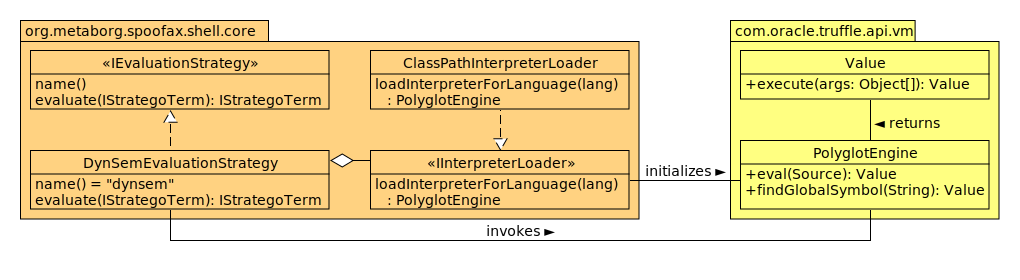
\includegraphics[width=0.8\textwidth]{uml-dynsem-eval-strat}
  \caption{UML diagram of the \texttt{DynSemEvaluationStrategy} and its
    collaborators.}
  \label{fig:uml-dynsem-eval-strat}
\end{figure}

%%% Local Variables:
%%% mode: latex
%%% TeX-master: "../main"
%%% End:


\section{ESV extensions}
\label{sec:esv-extensions}

To configure language specific features, such as the backend used to specify
the dynamic semantics of a language (see \cref{sec:eval-strat}) and the start
symbols valid within the context of a REPL, some REPL-specific extensions have
been made available in the ESV language.

\begin{lstlisting}[language=esv,caption={Configuring language specific settings.},label={lst:eval-method}]
module editor/SL-Shell

shell
    evaluation method : "dynsem"
    shell start symbol : Expr
    command prefix : ":"
\end{lstlisting}

The newly added configuration settings are illustrated in \cref{lst:eval-method}.
After loading a language that defines these additional settings, they will
be available via the ShellFacet, available through the language implementation.


\section{Dependency Injection}
\label{sec:injection}

The design of Spoofax makes extensive use of dependency injection, specifically
by using the Guice framework\footnote{\url{https://github.com/google/guice/wiki/Motivation}}.
To achieve as much interopability as possible, the final product
uses dependency injection in the same manner as Spoofax. Guice had a
substantial impact on the design and implementation of the final product, since
it nearly eliminates the need to create factories for complex datatypes.

Guice requires the programmer to bind implementations of dependencies in its
module classes, thereby separating behavior and dependency resolution.  Complex
datatypes can then accept their dependencies as constructor arguments, allowing
Guice to resolve and inject an instance of a bound type.

In the final product dependency injection is also used to supply classes
with a default configuration.  An example is the default list of commands
available to a user as described in \cref{sec:commands}.  The list of commands
is created from a Guice module by instantiating a \texttt{MapBinder} with
predefined bound commands. Child modules can then append extra entries to the
\texttt{MapBinder}, which makes them directly available to the existing
architecture.

Using dependency injection has made it easier to create a modular product,
centered around smaller interfaces interacting with each other. All these
interfaces can easily be bound to new implementations, thereby extending the
functionality of the REPL.


\section{Frontends}
\label{sec:frontends}

\Cref{cha:design} showed that the backend places few restrictions on the
frontends. A good example of this fact is the visitor pattern (see
\cref{sec:visitor}), which allows the frontends to schedule the processing of
the results and to display them in many different ways.  To illustrate this
flexibility, two frontends have been developed that operate on two different
spectra: a single threaded, text-based console frontend and a multithreaded
plugin to the Eclipse IDE. Both of these are discussed next.

\subsection{Console REPL}
\label{ssec:consolerepl}

The console REPL provides the user with a text-based user interface. For users
already accustomed to the command line, this is perhaps the most familiar
looking interface. A REPL running in the console requires a means of getting
user input from the standard input stream and printing results and error
messages to the standard output and error streams.

An excellent, BSD-licensed library that features these requirements is JLine2.
JLine2 is a library for handling console input, similar to GNU readline and BSD
editline. Most of the editing features present in these two libraries are also
present in JLine2.

\begin{figure}[h]
  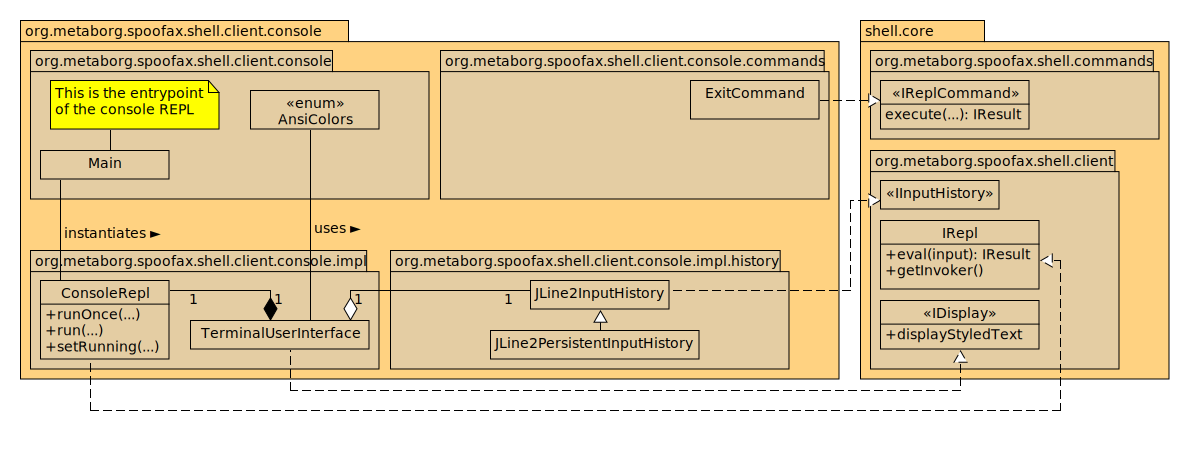
\includegraphics[width=\textwidth]{uml-console}
  \caption{UML diagram for the console frontend.}
  \label{fig:uml-console}
\end{figure}

As can be seen in \cref{fig:uml-console}, a frontend has to implement only a few
interfaces. The \texttt{ConsoleRepl} class is the central element in the
console frontend. It is instantiated first and controls the lifecycle of this
frontend. Its \texttt{run} method maps to the \texttt{loop} step in
Read-Eval-Print Loop and thus contains the \texttt{read}, \texttt{eval} and
\texttt{print} steps.

The \texttt{read} and \texttt{print} steps are provided
the by \texttt{TerminalUserInterface} class, which, as the name implies, is
responsible for the user interface. This class has connections to the standard
input, output and error streams. It uses JLine2 to provide a blocking input
editor. Because the input editor is blocking, the console REPL can run in a
single thread, thereby greatly simplifying its implementation.

A straightforward algorithm to provide multiline editing capabilities is used in
combination with JLine2's input buffer, which JLine2 does not natively support.
JLine2 does support input history, which means only an adapter class,
\texttt{JLine2IputHistory} had to be made to interoperate with the history
interface that is offered by the backend. An extension to this class is provided
to maintain persistent history.

To provide syntax and error highlighting, ANSI color codes are used. These
color codes are obtained through the \texttt{AnsiColors} enumeration, which
maps colors as returned by the \texttt{IResult} interface to their closest
ANSI equivalent.

Lastly, an \texttt{ExitCommand} is provided to halt the \texttt{run} method
in \texttt{ConsoleRepl}.

\subsection{Eclipse plugin}
\label{ssec:eclipse-plugin}

Spoofax currently features extensive integration in the Eclipse IDE. The client
expressed their interest to have this same level of integration for the REPL. A
plugin to the Eclipse IDE has been developed, which exposes the REPL
functionality through a graphical user interface that is familiar to anyone
working in Eclipse.

As is customary for a graphical user interface toolkit, the toolkit offered by
Eclipse uses multiple threads. One such thread is designated the ``UI thread'',
or user interface thread. This thread is responsible for processing
user-generated events (such as mouse clicks) and updating the graphical
representation of the widgets. All tasks that perform long running
calculations are supposed to be run in a background thread, such that the UI
thread is free to process incoming events. Instead, if a long running
computation is run in the UI thread, the widgets on the screen stop responding
to the user and the program appears to be in a frozen state. For this reason,
the backend has to perform its evaluations in a background thread, whilst all
the widgets and user interaction takes place in the UI thread.
The following discussion refers to the UML as depicted in
\cref{fig:uml-eclipse}.

\begin{figure}[h]
  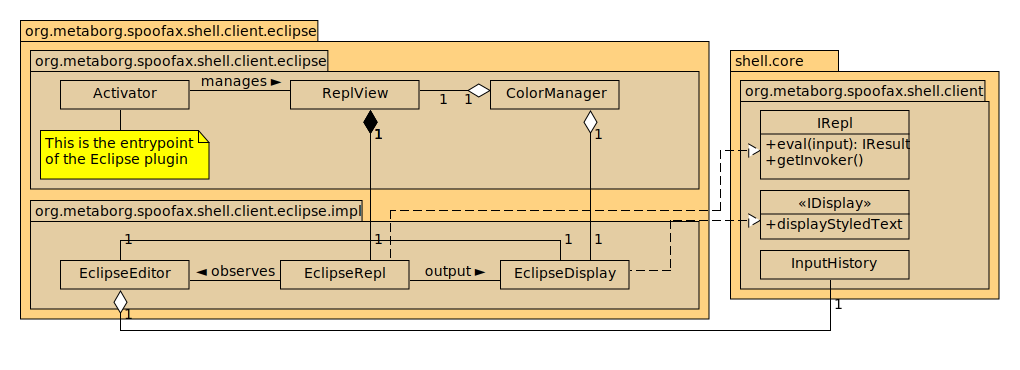
\includegraphics[width=\textwidth]{uml-eclipse}
  \caption{UML diagram for the Eclipse plugin.}
  \label{fig:uml-eclipse}
\end{figure}

Again, as can be seen in the UML, only a few interfaces have to be implemented.
The \texttt{EclipseRepl} class is the central element in the Eclipse plugin.
It is instantiated by the \texttt{ReplView} class, which in turn is
instantiated by Eclipse when the user requests the REPL to be opened. This
\texttt{ReplView} class also instantiates the input editor widget,
\texttt{EclipseEditor} and the \texttt{IResultVisitor} implementation,
\texttt{EclipseDisplay}.
In a multithreaded graphical user interface environment, asking text entry
widgets for the entered text is rarely a blocking process. This is no different
in Eclipse. For this reason, the \texttt{EclipseRepl} cannot simply loop as the
console REPL does. The solution is to use reactive programming through RxJava:
the \texttt{EclipseRepl} is registered as an observer to the
\texttt{EclipseEditor}. Then, when the user presses the Return key,
\texttt{EclipseEditor} notifies \texttt{EclipseRepl} with the contents of its
text buffer. \texttt{EclipseRepl} in turn launches a background job in which the
evaluation takes place, so as to not block the UI thread. Since the backend
simply returns an implementation of the \texttt{IResult} interface (see
\cref{sec:visitor}), the \texttt{EclipseRepl} can schedule the processing of this
result by the \texttt{EclipseDisplay} class on the UI thread. This processing
has to be done on the UI thread, because otherwise the \texttt{EclipseDisplay}
cannot update the widget it maintains to display results.
As one can see, the Eclipse plugin does not implement the \texttt{loop} step of
a REPL. There is no need to do so, due to the use of multithreading and reactive
programming.

%%% Local Variables:
%%% mode: latex
%%% TeX-master: "../main"
%%% End:


%%% Local Variables:
%%% mode: latex
%%% TeX-master: "main"
%%% End:


\chapter{Evaluation}
\label{cha:evaluation}

Two evaluations are made in this chapter. The first section of this chapter,
\cref{sec:product-evaluation}, evaluates the product. This is done firstly by
looking at the requirements and secondly by looking at the design goals, both as
described in \cref{sec:requirement-analysis}. The end of this section concludes
with an evaluation of the product as a whole in \cref{ssec:eval-product}. The
second section of this chapter, \cref{sec:process-evaluation}, evaluates the
process by which the product came to be. It discusses the development
methodologies used and the feedback as received by the Software Improvement
Group.

\section{Product Evaluation}
\label{sec:product-evaluation}

\Cref{sec:requirement-analysis} describes the requirements and the design goals
that were agreed upon with the client at the start of the project. This section
evaluates how these are met by the product. \Cref{ssec:eval-requirements}
discusses each requirement and decides whether or not it has been met and how.
\Cref{ssec:eval-design-goals} does the same for the design goals.  Finally, this
section concludes with a short discussion to see if the minimal viable product
as defined in \cref{ssec:mvp} has been delivered.

\subsection{Evaluation of the requirements}
\label{ssec:eval-requirements}

This section discusses all the requirements as set out in
\cref{ssec:requirements}. All the ``must have'', ``should have'' and ``could
have'' requirements are listed in \cref{table:requirements}. Per requirement,
the table lists whether it has been met, including an explanation as to how it
has been met or why it has not been met.

\begin{table}[]
\centering
\resizebox{\textwidth}{!}{%
\begin{tabular}{|l||l||l|}
\hline
\textbf{Requirement} & \textbf{Met?} & \textbf{Explanation} \\ \hline
Interactive REPL     & Yes           & \begin{tabular}[c]{@{}l@{}}Two interactive REPLs have been created: one for the console\\
								  and another in Eclipse.\end{tabular}\\ \hline
\begin{tabular}[c]{@{}l@{}}Works with any language\\ defined in
Spoofax\end{tabular} & Yes           & \begin{tabular}[c]{@{}l@{}}The backend retrieves the information it needs from Spoofax's\\
								  services. A language developer is able to define REPL-specific\\
					  			  configuration in an ESV file, as well.\end{tabular} \\ \hline
Input history        & Yes           & \begin{tabular}[c]{@{}l@{}}An interface with a corresponding client-agnostic implementation\\
								  has been created in the backend, allowing frontends to either use\\
								  the implementation or implement the interface as they see fit.\\
				  				  Both the console and the Eclipse frontend provide input history.\end{tabular} \\ \hline
\begin{tabular}[c]{@{}l@{}}Automatic binding of\\
previously yielded values\end{tabular} & Yes & \begin{tabular}[c]{@{}l@{}}The language designer can specify these semantics in DynSem.\end{tabular} \\ \hline
Multiline input editing                & Yes & \begin{tabular}[c]{@{}l@{}}The way in which input is given is not enforced by the backend.\\
									  However, both the console and the Eclipse frontend implement\\
					  				  multiline input editing.\end{tabular}\\ \hline
Error reporting      & Yes           & \begin{tabular}[c]{@{}l@{}}Both the console and the Eclipse frontend print errors to the user.\\
								  The characters to which these errors belong are highlighted in red.\\
							  	  Error reporting is not yet enabled during typing.\end{tabular}\\ \hline
Syntax-checked expressions             & Yes & \begin{tabular}[c]{@{}l@{}}The backend parses the input with the services provided by Spoofax.\\
							  		  As such, syntax-checked input was given for free. However, this\\
								  	  feedback is not yet enabled during typing.\end{tabular}\\ \hline
Syntax highlighting & No             & \begin{tabular}[c]{@{}l@{}}A working prototype has been implemented. Due to the nature of\\
								  console-based user interfaces, the console frontend cannot support\\
								  this feature. The Eclipse frontend has most of the required\\
							   	  functionality.\end{tabular}\\ \hline
Integration with Eclipse               & Yes & \begin{tabular}[c]{@{}l@{}}A REPL has been implemented in Eclipse, allowing the user to give\\
							  		  input and see output.\end{tabular}\\ \hhline{|=|=|=|}
Ability to redefine identifiers        & Yes & \begin{tabular}[c]{@{}l@{}}The language designer can specify these semantics in DynSem.\end{tabular} \\ \hline
Environment inspection                 & No  & \begin{tabular}[c]{@{}l@{}}This is impossible to do in the current DynSem implementation,\\
								  	  because the environment is captured in an object of type \texttt{Object}\\
								  	  and is therefore unprintable.\end{tabular} \\ \hline
Save and load REPL state               & No  & \begin{tabular}[c]{@{}l@{}}Due to limitations in time, this feature has not been implemented.\end{tabular}\\ \hhline{|=|=|=|}
Syntactic code completion              & No  & \begin{tabular}[c]{@{}l@{}}Spoofax's code completion services do not yet work with all\\
								  	  languages and are in process of a rewrite. As such, code\\
								 	  completion has not been attempted.\end{tabular}\\ \hline
\begin{tabular}[c]{@{}l@{}}Hover over variables to see\\
value, type and others\end{tabular}    & No  & \begin{tabular}[c]{@{}l@{}}Due to limitations in time and the fact that the environment is\\
					    			          captured in an object of type \texttt{Object}, this feature has\\
									  not been implemented.\end{tabular}\\ \hline
Literate programming                   & No  & \begin{tabular}[c]{@{}l@{}}An attempt has been made at writing an IPython frontend for the\\
								 	  REPL backend. However, due to limitations in time and the pressure\\
								  	  of finishing more important features, this work has not been finished.\end{tabular} \\ \hline
\begin{tabular}[c]{@{}l@{}}Integration with other\\
IDEs (IntelliJ)\end{tabular}           & No  & \begin{tabular}[c]{@{}l@{}}The Eclipse frontend is not entirely done yet, which was a\\
									  requirement before starting on implementing a frontend for\\
									  IntelliJ. As such, this feature has not been attempted.\end{tabular}\\ \hline
\end{tabular}
}
\caption{Evaluation of the requirements, separated per MoSCoW category.}
\label{table:requirements}
\end{table}

\subsection{Evaluation of the design goals}
\label{ssec:eval-design-goals}

In this section the design goals as set out in \cref{ssec:goals} are
discussed. Each design goal is listed below, along with an explanation as to how
it has been met.

\paragraph{Language-agnostic} This design goal stated that the REPL should work
for any language. Additionally, the language designer should be provided with a
language-agnostic interface to configure and implement the language-specific
parts of the REPL.

An extension of Spoofax's Editor Services has been created, allowing language
designers to configure certain parts of the REPL. Additionally,
language-specific changes, such as the ability to redefine identifiers, can be
made through DynSem. Currently, however, only DynSem-based interpreters are
supported, as opposed to Java- and Stratego-based interpreters. Despite this,
care has been taken to make this easily extendable. This design goal, therefore,
is met.

\paragraph{Minimal configuration} This design goal stated that the REPL should
require as little configuration as possible by reusing existing components of
the language definitions and automatically deriving other settings.

The extension of the Editor Services discussed in the previous design goal is
minimal. Three settings can be configured at the time of writing, all of which
have sane default settings. One additional setting is mandatory and cannot be
derived automatically (see \cref{ssec:supp-diff-ways}): the name of the
evaluation strategy to use. Additionally, because the existing DynSem
specification can be reused, only a minimal amount of new DynSem rules have to
be written to specify REPL-specific semantics. Finally, the SDF3 configuration
is reused to specify which start symbols are valid in case the language designer
wants to allow different start symbols. Therefore this design goal is met.

\paragraph{Maintainability} This design goal stated that the code should be
maintainable, because ownership will be transferred to the people already
working on Spoofax.

Various static analysis tools, up-to-date documentation, proper software design
and a received 4,5 out of 5 stars during the first round of feedback from the
Software Improvement Group (see \cref{ssec:sig} below), are good indications that
this design goal is met.

\paragraph{IDE-agnostic} This design goal stated that the REPL should place no
assumptions on the environment it runs in, since an effort is underway to do the
same for Spoofax itself.

The backend is agnostic to any frontend, no assumptions are made whatsoever:
console or graphical, blocking or unblocking user input, single- or
multithreaded, et cetera. This design goals is met.

\paragraph{Performance} This design goal stated that the REPL should be
performant, because care is taken to ensure that Spoofax itself is performant.

Launching the REPL is near instantaneous. Commands and expressions are evaluated
in real time, without noticeable delay. This design goals is thus met.

\paragraph{Modify Spoofax's existing codebase as little as possible} This design
goal stated that the REPL should be an extension to Spoofax, which means that
the existing codebase should be modified as little as possible.

The REPL is developed into a standalone repository. It uses the same API exposed
by Spoofax as any other extension would use. Minimal changes have been made to
Spoofax itself: the only large change that went upstream is the ability to
configure the REPL in an ESV file. However, DynSem had to be significantly
modified after its rewrite to support the use case of a REPL. These changes were
made in cooperation with its maintainer, and most were features that had to be
implemented regardless. As such, this design goal is also met.

\subsection{Evaluation of the product}
\label{ssec:eval-product}

This section evaluates whether the minimal viable product, as defined in
\cref{ssec:mvp}, has been delivered. The minimal viable product has been defined
as all the ``must have'' requirements (see \cref{ssec:requirements}), including
the design goals of being language-agnostic and having a minimal configuration.

The previous section concluded that all the design goals have been met.
\Cref{ssec:eval-requirements} and \cref{table:requirements} show that all the
``must have'' requirements have been implemented, except one: syntax
highlighting. The backend is ready to provide this functionality, and a working
prototype has been developed.

It is currently impossible to provide syntax highlighting in the console
frontend. The text-only environment is the limiting factor: once text has been
printed, it cannot be changed. This means that text would have to be printed
twice: once as it is typed in by the user, and again with syntax highlighting
applied.

The Eclipse frontend has the required functionality to provide syntax
highlighting. The backend, however, has no way of telling which widget (see
\cref{fig:frontend-eclipse}) to send the resulting text to. This means that as
of yet, only text in the output buffer can be highlighted.

As one might conclude, much of the code to implement syntax highlighting is
present. Finishing this work would not take much more effort. As such, this must
have requirement is close to being met. The minimal viable product is therefore
deemed to be delivered.

\section{Process Evaluation}
\label{sec:process-evaluation}

This section gives an evaluation of the process by which the delivered product
came to be. First, the methodologies used during development are discussed in
\cref{ssec:dev-meth}. \Cref{ssec:sig} shows the feedback received from the
Software Improvement Group and discusses the changes that were made to the code
accordingly.

\subsection{Development methodologies}
\label{ssec:dev-meth}

In the beginning of the project, agreements were made on the development
methodologies that were to be used. Throughout the duration of the project, some
of these methodologies turned out to work well, whilst others were less
effective than anticipated. This section discusses these agreements.

The Scrum methodology was chosen to manage the product development. Previous
experience showed that one week sprints are often too short, so for this project
biweekly sprints were decided. This worked well: there was enough time to make
informed decisions and to evaluate or rework certain things. Biweekly sprints
also allow for an easier revision for the sprint plan if changes need to be
made due to unexpected issues.

Sprints were evaluated with a meeting with the client, during which the progress
was demonstrated. The feedback received during these meetings was valuable and taken
into account to guide the next sprint.

The client mandated the use of Trello to manage the sprints, which has been a
positive experience as well. Trello makes it easy to manage deadlines and to
know what has to be done at what time. Managing a backlog of user stories and
moving them around from, for example, ``developing'' to ``testing'', is
straightforward and helps to keep everyone, including the client, updated on the
progress.
The pull-based development model worked well, as was anticipated from previous
experience. The continuous integration, in combination with a set of strict
static analysis tools, ensured that the code review process had a positive
influence on the quality of the code.\\

Naturally, there were also things that could have gone better. It is easy to
underestimate the amount of work when putting together a sprint plan, which has
been a source of problems. The solution for this issue is to deliberately plan
less: it is easier to move new user stories to the sprint plan than it is to
decide which user stories not to complete.

A second issue concerns the unstable development environment provided by Eclipse.
Omitting all the details, several hard to track issues occurred which took a
considerable amount of time to resolve. To add to this, on several occurrences
the development of the Eclipse plugin had to wait for changes to make it into
Spoofax.

The biggest issue that occurred during the development is the fact that Spoofax
is a moving target. Halfway through the allotted time for development, DynSem
was significantly rewritten. After this rewrite, the functionality required for
a REPL was no longer present. To resolve this, considerable effort has been spent
to add these features to DynSem in cooperation with DynSem's maintainer. All of
this work has been accepted upstream and has now been published in the latest
snapshot releases.\\

To conclude, the process by which the product came to be went predominantly
well, despite some issues that can be improved during future projects.

\subsection{Software Improvement Group}
\label{ssec:sig}

The code was sent to the Software Improvement
Group\footnote{\url{https://www.sig.eu/}} for review on May 27th. The following
feedback was received on the third of June:

\begin{quotation}
[Analyse]

De code van het systeem scoort 4,5 ster op ons onderhoudbaarheidsmodel, wat
betekent dat de code bovengemiddeld onderhoudbaar is. De hoogste score is niet
behaald door een lagere score voor Unit Interfacing.

Voor Unit Interfacing wordt er gekeken naar het percentage code in units met een
bovengemiddeld aantal parameters. Doorgaans duidt een bovengemiddeld aantal
parameters op een gebrek aan abstractie. Daarnaast leidt een groot aantal
parameters nogal eens tot verwarring in het aanroepen van de methode en in de
meeste gevallen ook tot langere en complexere methoden.

In jullie geval heeft de constructor van \texttt{Data} een enorm aantal
parameters. Er zijn grofweg twee manieren om dat te addresseren: de eerste is
het groeperen van velden in sub-types. Een flauw voorbeeld is het groeperen van
\texttt{width} en \texttt{height} in een type \texttt{Dimensions}.
Dit voorbeeld is natuurlijk triviaal, maar je ziet wel vaak dat studenten aan
het begin wat huiverig zijn om kleine classes voor alleen een type te
introduceren, terwijl dit op de lange termijn vaak wel degelijk zin heeft. De
tweede manier is niet meer alle parameters in de constructor meegeven, maar via
setter-methodes. Dat leidt tot meer code, maar maakt het intialiseren van een
object wel leesbaarder.

Een ander voorbeeld van dezelfde situatie is de constructor van
\texttt{TransformCommand} (zo te zien krijgen jullie daar ook al een
waarschuwing vanuit CheckStyle). Dit geval is wat moeilijker op te lossen,
aangezien jullie hier van dependency injection gebruik maken en de methode
daardoor wat moeilijker kunnen refactoren.

Het is goed om te zien dat jullie naast productiecode ook veel testcode hebben
geschreven. De verhouding tussen de hoeveelheid productiecode en testcode is met
bijna 1 op 1 ook zeer gezond. Hopelijk lukt het jullie om dat vast te houden
tijdens het vervolg van het project.
\end{quotation}

This analysis says that the code scored bad on unit interfacing, because there
were quite a few classes that had an above average amount of constructor
parameters. The reason that this came to be is the fact that dependency
injection is used, as opposed to the traditional way of managing dependencies.
This fact is also mentioned in the analysis itself.

Two suggestions were given as a possible solution to this problem: create new
classes that encapsulate several parameters, or use \texttt{setter} methods
to pass parameters this way. However, neither solution was satisfactory as-is:
data classes are often considered to be a code smell, and \texttt{setter}
methods risk not fully initializing an object. The classes to which the
criticism applied have been refactored into smaller, more manageable units.
Ultimately, this not only led to resolving the only negative feedback made by
the Software Improvement Group, it also led to a better architecture.

%%% Local Variables:
%%% mode: latex
%%% TeX-master: "main"
%%% End:


\chapter{Discussion and Recommendations}
\label{cha:disc-recomm}

In this chapter the achieved results will be discussed, as well as some tasks
that were not achieved. In \cref{cha:evaluation} we have already discussed how
our final product satisfied the customers requirements. Here it will be
discussed why not all these requirements have been met. Afterwards some
recommendations will be outlined regarding the changes that should be made to
both the REPL and to Spoofax in order to meet them. Finally some
recommendations regarding possible directions for future work will be given.

\section{Discussion}
\label{sec:discuss-discussion}

\subsection{Language interpreters have to be on the classpath}
\label{sec:discuss-classpath}

\subsection{String representation of Dynsem data types}
\label{sec:discuss-dynsem-string


\section{Recommendations}
\label{sec:discuss-future}

\subsection{Implementing an IPython kernel for Jupyter notebooks}
\label{sec:literate-programming}

As explained in \cref{sec:a-literate-programming}, IPython (together with
Jupyter notebooks) supports both reproducible research and literate
programming. The client had expressed his interest in literate programming
functionality for Spoofax. Implementing an IPython kernel on top of the core
shell module should not take a lot of effort, however due to the problems
discussed earlier priority was given to a solid working REPL and an Eclipse
plugin. Therefore our product does not deliver an implementation of literate
programming.

IPython kernels provide a solid framework for literate programming that has
proven itself in many different languages
\footnote{https://github.com/ipython/ipython/wiki/IPython-kernels-for-other-languages}.
An IPython kernel is basically a daemon with several network sockets
representing the in and output streams of the client application. Several
message types are sent over these sockets in JSON format, such as requests to
evaluate a certain string or requests regarding the kernel
state\footnote{https://jupyter-client.readthedocs.io/en/latest/kernels.html}.

Since the invoker class from the core module just accepts any string given to
it and then resolves the command itself, implementing an IPython kernel should
be pretty straightforward. Most of the required work would be in creating an
adequate messaging framework capable of understanding all defined JSON
messages. When the messaging framework is in place user input can be sent
directly to the invoker and results can be displayed using the ``IResult''
interfaces as with any other client implementation.

\begin{figure}[htb]
  \centering
  \includegraphics[width=\textwidth]{ipython}
  \caption{A plot from data in an IPython notebook.}
  \label{fig:ipython}
\end{figure}

By implementing an IPython kernel all functionality offered by Jupyter
notebooks (see \cref{fig:ipython}) would be available to the Spoofax REPL at
once. This would directly result in the ability to live edit code interspersed
with documentation, while also allowing more complex graphical elements.

%%% Local Variables:
%%% mode: latex
%%% TeX-master: "../main"
%%% End:


%%% Local Variables:
%%% mode: latex
%%% TeX-master: "main"
%%% End:


\chapter{Conclusion}
\label{cha:conclusion}

Over the course of the last quarter the Spoofax Language Workbench has been
explored and a Read-Eval-Print Loop (REPL) has been created that operates with
any language defined in the Spoofax.

\Cref{cha:background} gave the required background knowledge needed to
understand the problem domain. \Cref{cha:probl-defin-analys} framed the problem
definition in the context of this background. \Cref{cha:design} and
\cref{cha:implementation} discussed the design and the implementation of the
final product. \Cref{cha:evaluation} evaluated both the final product and the
process by which it came to be. \Cref{cha:discussion} reflected upon the
project, after which \cref{cha:recommendations} made recommendations to improve
the final product.

To successfully complete the project, extensive knowledge needed to be gained of
the conceptual ideas behind programming language implementations, and of the
Spoofax API implementing these concepts.

Once the required knowledge was attained, two contributions have been
made. First, a functioning REPL has been created,
comparable in features to those of popular programming languages such as Python
and Haskell. Second, changes have been contributed to Spoofax that
have been integrated into the main repository.

Despite having faced significant challenges during the start of the project, the
most important goals as set forth in the problem description have been achieved.
Therefore, the project team is still satisfied with the end result: while
not all requested features have been implemented, it has been shown that it is
possible to create a functioning REPL for any language defined in Spoofax,
requiring only additional configuration to a language definition.

%%% Local Variables:
%%% mode: latex
%%% TeX-master: "main"
%%% End:


\appendix

\bibliography{references}{}

\chapter{Project Description}
\label{cha:project-description}
\addtocontents{toc}{\protect\setcounter{tocdepth}{0}}

\paragraph{Create a command-line shell interface for the Spoofax Language
Workbench}\mbox{}\\

From Spoofax's website:

\begin{quotation}
Spoofax is a platform for developing textual domain-specific languages with
full-featured Eclipse editor plugins.
\end{quotation}

A feature that Spoofax is lacking is a Read-Eval-Print Loop (REPL). A REPL is an
interactive programming environment that takes expressions, evaluates them and
prints their results. REPLs are a popular tool for programming because they
facilitate exploratory programming and debugging. Common examples include
command-line shells such as Bash and Python's REPL.

The deliverable for this project, then, is to create such a REPL for the Spoofax
Language Workbench.

%%% Local Variables:
%%% mode: latex
%%% TeX-master: "main"
%%% End:


\chapter{Research Report}
\label{cha:research-report}
\addtocontents{toc}{\protect\setcounter{tocdepth}{0}}

\section*{Introduction}
\label{sec:introduction}
\addcontentsline{toc}{section}{Introduction}

Spoofax is a language workbench developed by Delft University of
Technology over the course of several years. During those years it has
grown to be \textit{``a language workbench for efficient, agile
  development of textual domain-specific languages with
  state-of-the-art IDE support''}~\cite{Kats10a}.

When developing new domain-specific languages using Spoofax, the
ability for rapid prototyping using a read-eval-print loop (REPL)
would be very convenient. This report describes the initial research
phase for this project: extending Spoofax with generating REPLs for the
languages defined with it.

The first three sections of this research report give an overview of
the problem domain. \Cref{sec:spoofax} gives the scope of Spoofax and
each of its meta-languages. In \cref{sec:repl}, REPLs are explained in
more detail. After that \cref{sec:literate-programming} introduces
literate programming.

The remaining four sections concern the problem and the project. In
\cref{sec:problem-definition}, a short problem definition is
given. \Cref{sec:problem-analysis} then gives an analysis of this
problem definition in the context of the services that Spoofax already
provides, to clarify potential problems and their solutions to
generate REPLs that work with languages defined in Spoofax. Next, in
\cref{sec:requirement-analysis}, a list of design goals will be
formalized to guide the development of the deliverable. From these
design goals and the problem definition and analysis, a list of
requirements for the product will be compiled. Lastly,
\cref{sec:realisation-product} gives an account of the development
frameworks and tools to be used during the development of the project.

%%% Local Variables:
%%% mode: latex
%%% TeX-master: "main"
%%% End:


\section{The Spoofax Language Workbench}
\label{sec:spoofax}
Spoofax is an environment that allows for the completely \emph{declarative}
definition of a programming language. The definition is done using
high-level \emph{meta-languages} for each aspect of the programming
language.

To define a language declaratively means that one uses the
meta-languages to specify \emph{what} the properties of a language are, and
not \emph{how} these properties are
implemented\footnote{Reference: Declare your language book
preface}. For example, instead of asking "How do I implement a
tokenizer and parser for my language?", one asks "What is the syntax
of my language?". From such a description in a meta-language, the
tokenizer and parser can be derived, without the designer of the
language ever having to care about its implementation.

This section goes over the elements that make up the specification of
a language using Spoofax:
\begin{enumerate}
\item \hyperref[sec-syntax-def]{Syntax Definition}: Specifying the syntax of a language.
\item \hyperref[sec-static-analysis]{Static Semantics}: Describing the static analysis part of a
language: type checking, name binding and variable scoping.
\item \hyperref[sec-term-rewrite]{Term Rewriting and Program Transformation}: Rewriting ASTs to new
ASTs, for example to declare desugaring rules.
\item \hyperref[sec-dynamic-semantics]{Dynamic Semantics}: Defining what the language does upon execution.
\end{enumerate}

The structure of this section follows that of the language
specification portion of the compiler construction course. The slides
of this portion of the course can be found here:
\url{http://tudelft-in4303.github.io/lectures/specification/}.
\subsection{Syntax Definition}
\label{sec-syntax-def}
The first part of Spoofax to consider is Syntax Definition. To specify
a syntax definition declaratively, a DSL called SDF3 is used. The
syntax definition can be used to make parsers which parse text to AST
and pretty-printers for mapping ASTs back to text. Furthermore, it can
be used for error recovery rules, syntax highlighting rules and
folding rules for editors.

All the other parts of Spoofax operate on the AST that is produced by
a parser generated from a SDF3 specification.
\subsection{Static Semantics}
\label{sec-static-analysis}
Static semantics refer to the meaning of what is a well-formed program
for a particular language~\cite{Milner97}. This imposes more
constraints than syntax definition, such as name binding, scoping
rules, and type checking. These cannot be specified by a syntax
definition alone, and are thus considered separately.
\subsubsection{Declarative Static Semantics Specification in Spoofax}
\label{sec:orgheadline1}
In Spoofax, all the static semantics as well as the dynamic semantics
used to be specified with the Stratego transformation language (which
will be discussed in \hyperref[sec-term-rewrite]{Term Rewriting}). Nowadays, two higher level DSLs
exist for specifying static semantic declaratively: NaBL and TS. The
two DSLs can work together: for instance, the type of a variable can
be set in NaBL, so that TS can make assertions on it.
\subsubsection{NaBL: the Name Binding Language}
\label{sec:orgheadline2}
With NaBL (pronounced \emph{enable}), name binding and scoping rules can be
specified. Here is an example of the name binding and scoping rules
for a class, from the paplj language:
\begin{verbatim}
namespaces Program Class Field Method Variable
// ...
binding rules
  Class(c, _, _, _) :
    defines Class c of type ClassT(c)
    // Declare new scope
    scopes Field, Method, Variable
    implicitly defines Variable This() of type ClassT(c)

  Extends(c) :
    // Import namespaces from superclass
    imports Field, Method from Class c
\end{verbatim}
The first line declares the namespaces to
consider. Then for each node in the AST resulting from the parsing,
for example a \texttt{Class} node, the name binding and scoping rules can be
defined. In the example, each \texttt{Class} node declares a new scope for
its fields, methods and variables. It also implicitly defines the
\texttt{this} variable. The \texttt{Extends} node can then import the fields and
methods into its scope.

As can be seen from line 8, it can also associate type information
with names, to interplay with TS. The type annotations can also be
used for instance when desugaring or rewriting with Stratego (see \hyperref[sec-term-rewrite]{Term
Rewriting}).
\subsubsection{TS: the Type Specification Language}
\label{sec:orgheadline3}
Type checking can be done with the TS DSL. Again an example of the
paplj language:
\begin{verbatim}
type rules
  Class(c1, Extends(c2), _, _) :-
    where store ClassT(c1) <sub: ClassT(c2)

  x@This() : t
    where definition of x : t
// ...
type rules
  Add(e1, e2) : NumT()
    where e1 : NumT() else error "number expected" on e1
      and e2 : NumT() else error "number expected" on e2
\end{verbatim}
Rules can recursively set constraints on AST-nodes, such as the \texttt{Add}
node in the above example.

Again, in line 5, interplay can be seen between TS an NaBL. Here the
type of a variable can be accessed, which is set in the NaBL
specification (see previous section).
\subsection{Term Rewriting and Program Transformation}
\label{sec-term-rewrite}
Spoofax offers a high level declarative DSL called Stratego for program
transformation. Stratego operates on ASTs, and is the most general
part of Spoofax: it can be used for static semantics (name binding,
type checking), desugaring and for the dynamic semantics of a
language.

As the static semantics can now be done using NaBL and TS, and the
dynamic semantics with DynSem (see next section), Stratego can be used
to specify desugaring rules for a language.

Stratego is based on the notions of \emph{term rewrite rules} and so called
\emph{strategies}.
\subsubsection{Rewrite rules}
\label{sec:orgheadline4}
A rewrite rule is a transformation on a term, in which
the left-hand side allows for pattern matching and variable binding,
and the right hand side instantiates new replacement terms. An example
of a rewrite rule is given below.
\begin{verbatim}
rules
  desugar-let :
  	Let([], e) -> e

  desugar-let :
  	Let([b1, b2 | bs], e) -> Let([b1], Let([b2 | bs], e))
\end{verbatim}
This desugars a \texttt{let} expression with multiple bindings into multiple
nested \texttt{let} expressions each having just one binding.
\subsubsection{Strategies}
\label{sec:orgheadline5}
Strategies are used to select and apply term rewrite rules, to
construct the main algorithm of the program transformation. One can
use multiple combinators to compose rewrite rules and other
strategies. An example is given below:
\begin{verbatim}
strategies
  pre-desugar =
    innermost(desugar-let <+ desugar-do)

  post-desugar =
    innermost(desugar-do <+ desugar-get <+ desugar-set);
    resugar
\end{verbatim}
For example, \texttt{innermost} is a strategy to apply the strategy given as
parameter (a composition of rewrite rules) on the innermost AST node,
and repeats this until the strategy is no longer applicable\footnote{Is
this correct?}.
\subsection{Dynamic Semantics}
\label{sec-dynamic-semantics}
Dynamic semantics refers to how a program in some language
behaves~\cite{Winskel93}. There are multiple approaches to
formally specify the dynamic semantics of a programming language (for
an extensive treatment, see~\cite{Winskel93}). For this section
only one sort of approach is relevant, namely \emph{rule-based operational}
\emph{semantics} (see~\cite{Plotkin04} for a historical account of this
approach).

\subsubsection{DynSem: a rule-based dynamic semantics}
\label{ssec-dynsem}
In Spoofax, the dynamic semantics of a language used to be specified
with Stratego. However, the Spoofax team has developed a more
high-level way to declare the dynamic semantics of a language, namely
a DSL called \emph{DynSem}~\cite{VerguNV15}. As with all DSLs in
Spoofax, DynSem offers a declarative approach to generate the
\emph{implementation} out of the \emph{specification}. Indeed, from a DynSem
specification of a language, an interpreter for that language can be
generated.

In DynSem, the dynamic semantics are specified by means of rules. To
show how rules can define the dynamic semantics of a language,
consider the classic example of the \(\beta\)-reduction, which defines
function application in the lambda calculus. The rule replaces all the
occurences of the parameter \(x\) with the argument \(e_2\), within the
expression \(e_1\):

\begin{equation}
(\lambda x.e_1) e_2 \rightarrow e_1[x := e_2]
\end{equation}

In a similar way, dynamic semantics can be specified in DynSem, in a
syntax very similar to the formal syntax used in the literature. Take
here the example of method calling in paplj:

\begin{verbatim}
rules
  // ...
  Call(o, m, vs: List(V)) --> v'
    where lookupMethod(o, m) --> Method(_, _, params, e);
          This o, Env bindVars(params, vs) |- e --> v'.
\end{verbatim}

The bottom line represents the rule of the method body, \(e\),
evaluating to the return value \(v'\), by binding the argument values to
the parameter in the environment and binding the \texttt{this} variable to
the object on which the method is called. Exactly how \(e\) evaluates to
\(v'\) is defined using other rules, which are left out in this example.


%%% Local Variables:
%%% mode: latex
%%% TeX-master: "main"
%%% End:


\section{Read-Eval-Print Loops}
\label{sec:repl}

Many programming languages come with an interactive environment. This
interactive environment is an interface to the programming language's execution
engine. One common form of such an environment is an interface in which
expressions in a programming language are typed by the user, after which the
results of that expression are printed back to the user. Such an environment is
called a Read-Eval-Print Loop (REPL), although many different names are known,
including but not limited to \textit{language shell},
\textit{command-line interpreter} or \textit{interactive interpreter}. There
are subtle differences between these names and the name REPL. These are,
however, mostly of semantic value. In this report the term REPL is chosen,
because it conveys the notion of such an interactive environment well.

\subsection{Origin of REPLs}
\label{repl-origin}

The Lisp programming language is one of the first programming
languages offering such functionality~\cite{Noyes92}. The name REPL comes from
the Lisp functions that implement it:

\begin{enumerate}
  \item The \texttt{read} function takes a user's input, which often is just one
    or several expressions as opposed to a complete compilation unit. It then
    parses this input and creates an abstract syntax tree (AST).
  \item The AST created in the previous step is then passed on to the
    \texttt{eval} function, which evaluates it.
  \item The result yielded by the previous function is then printed out to the
    user by the \texttt{print} function.
  \item After having printed the result, the environment needs to \texttt{loop}
    back to the read state.
\end{enumerate}

Assuming the individual functions listed previously exist, a REPL can be created
in a single line of code simply by combining the functions:

\begin{lstlisting}[language=lisp]
(loop (print (eval (read))))
\end{lstlisting}

Part of the semantic differences between the different names for an interactive
programming environment is Lisp's homoiconicity. In Lisp, the structure of
expressions is represented directly in a data structure, resulting in the
ability to infer a program's or data object's state simply by reading its
textual representation. In Lisp REPLs, therefore, arbitrary data objects yielded
from a previous expression can be used as input to the next expression. In
modern programming languages that do not belong to the Lisp familiy,
homoiconicity is an unusual feature. Interactive environments for these
languages therefore often require additional steps to read and evaluate
expressions. As said earlier, this difference is mostly semantic and therefore
this report uses the more general interpretation of the name REPL.

\subsection{Advantages of REPLs}
\label{ssec:repl-advantages}
REPLs offer several advantages that make them an often requested feature.
Because of their nature, REPLs provide the ability to program interactively.
Programming interactively has multiple applications.

When creating software solutions for an as of yet not well understood domain,
it is often not clear which data structures and algorithms are required. In such
cases, REPLs offer the ability to interactively develop and debug software
without having to apply the (oftentimes much slower) edit-compile-run-debug
development style. This kind of programming is called exploratory
programming~\cite{Fritzson86}. Related to this kind of exploration, REPLs also
provide a means for rapid prototyping and bottom up programming~\cite{Graham93}.

The explorative and interactive features of a REPL also make it an excellent
tool for programmers to learn a new programming language. REPLs are also
combined with what is called literate programming to offer notebooks or language
playgrounds, as discussed in~\cref{sec:literate-programming}.

\subsection{Functionality}
\label{sssec:repl-functionality}

Every programming language providing a REPL has its own set of functionality.
However, a core set of functionalities, shared between all REPL implementations,
can be identified. To reach this core set of features, well-known REPLs have
been investigated and their features have been compiled into a matrix as seen
in~\cref{table:feature-matrix}. These features are shortly discussed below.

\todo{Make~\cref{table:feature-matrix} complete. At the very least, make the
partially filled in columns complete. If time allows, look into the as of yet
open columns}
\begin{table}[]
\centering
\begin{tabular}{lccccccccc}
                                  & \rot{Python} & \rot{R} & \rot{\shortstack[c]{Common\\Lisp}} & \rot{Haskell} & \rot{Swift} \\
\toprule
Executes single expressions       & \cmark       & \cmark  & \cmark                             & \cmark        & \cmark      \\
Executes statements               & \cmark       & \cmark  & \cmark                             & \cmark        & \cmark      \\
Input \& output history           & \cmark       & \cmark  & \cmark                             & \cmark        & \cmark      \\
Persistent input history          & \cmark       & \cmark  & \xmark                             & \cmark        & \cmark      \\
Multiline input editing           & \cmark       & \cmark  & \cmark                             & \cmark        & \cmark      \\
Redefining identifiers            & \cmark       & \cmark  & N/A                                & \cmark        & \cmark      \\
Error reporting                   & \cmark       & \cmark  & \cmark                             & \cmark        & \cmark      \\
Context-sensitive code completion & \cmark       & \xmark  & N/A                                & \xmark        & \cmark      \\
Help or documentation system      & \cmark       & \cmark  & \cmark                             & \xmark        & \xmark      \\
Additional commands to the REPL   & \xmark       & \xmark  & \cmark                             & \cmark        & \cmark      \\
Nested REPLs to enable debugging  & \xmark       & \xmark  & \cmark                             & \xmark        & \xmark      \\
\bottomrule
\end{tabular}
\caption{A feature comparison of several well-known REPLs}
\label{table:feature-matrix}
\end{table}

\paragraph{Input \& output history} REPLs keep a history of inputs and outputs,
such that previously entered expressions can be retrieved together with their
(evaluated) results. This can be with, say, a keyboard shortcut to retrieve
prevsiouly entered inputs and with variables bound to previously yielded values.

\paragraph{Persistent history} The input and output history as discussed
previously can be recorded into a file (either per-project or globally) to
enable a persistent history of input and output.

\paragraph{Multiline input editing} Constructs in a programming language are
not necessarily bound to one line; a method in Java for example often has the
following structure:
\begin{lstlisting}[language=java]
boolean isEven(int number) {
    return (number % 2) == 0;
}
\end{lstlisting}
One should be able to type these constructs in their habitual way. Therefore,
REPLs provide multiline input editors that recognise incomplete code and
promptly switch to a multiline environment when required.

A REPL is just another programming environment; just as in a regular editor or
IDE, therefore, keyboard shortcuts should be present to improve the workflow of
the programmer. This includes keyboard shortcuts to move over words, delete
words (both in forward and backward directions) and jump to the beginning or
end of the line.

\paragraph{Redefining identifiers} When using a REPL in an exploratory manner,
it is not uncommon to want to redefine an identifier's type or to completely
reimplement a method. In this way, a REPL can be different than its host
language, especially if the host language is a functional language that doesn't
allow variable's values to change once initiated.

\paragraph{Error reporting} A REPL should provide the same error reporting
capabilities as an IDE; preferably while typing input but at the very least it
should be able to report errors during the reading and evaluation phases.

\paragraph{Context-sensitive code completion} Context-sensitive code completion
is a helpful tool to provide an overview of the often many APIs a developer
works with, freeing them from having to remember everything. Note that this is
distinct from general tab-completion, which is not context-sensitive and is
offered by all the studied REPLs.

\paragraph{Help or documentation system} The exploratory nature of a REPL means
that one will often see new methods. It would be helpful to read one or several
lines of documentation in case it is required, so that the developer does not
have to switch contexts.

\paragraph{Additional commands to the REPL} Some REPLs offer additional
commands to inspect the environment or to control their behavior. These commands
are oftentimes not in the syntax of the language the REPL belongs to and are
highly diverse REPL implementations. A notable example of a REPL offering such
commands is Haskell's GHCi~\cite{GHCi-commands}.

\paragraph{Nested REPLs to enable debugging} A notable feature of (mostly) Lisp
REPLs is that in case of an error, a new REPL is spawned inside the context of
this error. This REPL then has additional commands (see the above feature) to
enable debugging and inspection of the error state. When the user has
resolved the error, the nested REPL exists and the user is returned to the
parent REPL. This can go to arbitrary depths.

%%% Local Variables:
%%% mode: latex
%%% TeX-master: "main"
%%% End:


\section{Literate Programming}
\label{sec:literate-programming}

%%% Local Variables:
%%% mode: latex
%%% TeX-master: "main"
%%% End:


\section{Problem Definition}
\label{sec:problem-definition}

The previous sections provided the necessary background knowledge of
the problem domain. Now that the background knowledge has been
explained, this section will discuss the problem definition of the
client.

Spoofax offers a wide variety of tools to develop DSLs and
accompanying IDE support. Precisely because Spoofax is concerned with
developing DSLs, rapid prototyping of syntax and grammar is a
convenient addition to the product. \Cref{sec:repl} showed that REPLs
provide this rapid prototyping ability for other languages like Lisp
and Python. Therefore, the client has expressed their interest in
REPLs that are generated from language definitions created with
Spoofax. Such a REPL would aid both the developer of the language, and
its end-user.

Since a lot of language services are already provided by Spoofax, the
REPL should try to hook into existing services as much as possible.
Besides exposing already existing Spoofax services in an interactive
shell, the product should also expose additional features geared
towards interactive exploration of programs in the generated
languages.  Examples include displaying and editing the contents of
current program context, saving and loading program context and
keeping a history of executed expressions.

When a REPL is realized, the product could be further extended to add
support for literate programming, allowing for rapid prototyping and
documentation at the same time~\cite{schulte2012}. This would allow
developers of new DSLs to document and explain their language in an
interactive manner that directly allows experimentation.

%%% Local Variables:
%%% mode: latex
%%% TeX-master: "main"
%%% End:


\section{Problem Analysis}
\label{sec:problem-analysis}


\subsection{Incorporating REPL generation within Spoofax}
\label{ssec:architecture}

\subsubsection{The relevant parts of Spoofax}
\label{sec:which-parts-spoofax}

\subsubsection{The available APIs from Spoofax}
\label{sec:what-are-available}

\subsection{Plug-in development in Eclipse}
\label{ssec:eclipse-plugins}

%%% Local Variables:
%%% mode: latex
%%% TeX-master: "main"
%%% End:


\section{Requirements Analysis}
\label{sec:requirement-analysis}

Defining requirements upfront is important for several reasons: it is a contract
between the developers and the client, it guides the product development, it
enables the client to track the progress and finally it allows validation of the
deliverable. These requirements are listed in this section.

\subsection{Design goals}
\label{ssec:goals}

The client has expressed some high-level requirements, which are listed in this
subsection as design goals in order of priority. The design goals serve as an
important guideline when defining and implement the invidual requirements. As
such, they can be considered the bounds within which all requirements must fit.

\paragraph{Language-agnostic} The REPL should work with all languages
defined with Spoofax. This means that no assumptions can be made about any
language constructs or syntax.

\paragraph{Autogeneration} The REPL should be automatically provided, just like
all of Spoofax's other services. This means that providing access to the shell
should be integrated into Spoofax's build system and not require any additional
steps from the user.

\paragraph{Maintainability} Spoofax is an already existing, open source project
managed by several people. When the product is delivered, it will have to be
maintained by others. Therefore, it is important that the code is maintainable.

\paragraph{Performance} Spoofax's developers already focus quite a bit on
performance: both the generation and the use of the services are performant.
This should be no different for the REPL.

\paragraph{Modify Spoofax's existing codebase as little as possible} The product
should be an extension to Spoofax, which means the changes made to the existing
Spoofax codebase should be as small as possible. Preferably, the REPL service
should be a standalone module.

\subsection{Requirements}
\label{ssec:requirements}

Under the guidance of the design goals listed in the previous subsection, the
requirements compiled from the feature matrix discussed in \cref{sec:repl} and
meetings with the client are discussed below, under the MoSCoW method.

\subsubsection{Must have}

Requirements listed under ``must haves'' are of critical importance to the
usability and success of the deliverable. Without these, the product is not in a
workable state and is not likely to be accepted by the client. \emph{Must} can
also be considered an acronym for the Minimum Usable SubseT.

\paragraph{Interactive shell} Per the definition of a REPL given in
\cref{sec:repl}, the REPL has to be interactive. It should evaluate single
statements and expressions typed in by the user and print the results back to
them.

\paragraph{Operates with language definition} Every service in Spoofax operates
from language definitions. It is evident that the REPL should work with these
definitions if it is to fit within Spoofax.

\paragraph{Input \& output history} Users should be able to retrieve previously
typed expressions and statements to support the explorative and interactive
nature of a REPL. In the same vein, previously yielded results should be
implicitly bound to automatically generated names to make their values available
in future expressions.

\paragraph{Multiline input editing} Most, if not all, modern languages benefit
by structuring their constructs over multine lines. Multiline input editing is
therefore a crucial feature for user satisfaction. The input editor should
start in single line editing mode and recognise when an expression or statement
is part of a multiline construction. When it recognises this, it should
automatically switch to its multiline input editing mode, wherein the
prompt character indicates this new mode. This mode's behavior (e.g. keyboard
shortcuts) is different from the single line editing mode.

\paragraph{Error reporting} To support the interactivity of the REPL, error
reporting should be available in two ways: while typing an expression or a
statement, on-the-fly error reporting should indicate wrongly typed items. The
interpreter that evaluates syntactically correct input should also be able to
display its error messages to the user in case of an error during the dynamic
semantics phase.

\paragraph{Syntax checked input} Supporting the above requirement, all
input should have its syntax checked on the fly.

\paragraph{Syntax highlighting} All expressions and statements (whether they are
currently being entered, displayed as previously entered input or displayed as
previously yieled results) should be syntax highlighted.

\paragraph{Integration with Eclipse} As first implementation, the REPL should
integrate with Eclipse to provide an interface to the users. It is important to
note that while integration with Eclipse is a requirement, Spoofax itself is
moving to be IDE-agnostic. As such, the implementation of the REPL's core
should not be tied to Eclipse.

\subsubsection{Should have}

Requirements listed under ``should-haves'' are important, but not necessary for
a working product.

\paragraph{Ability to redefine identifiers} As explained in \cref{sec:repl},
REPLs provide the ability to explore unknown problem domains. It is not a
far-fetched idea that a developer would want to change function implementations
or the types of certain variables. To support this, a REPL should allow users to
redefine identifiers. This might mean that the REPL needs different semantics
than the language it operates on, slightly contrasting the requirement that the
REPLs should be language-agnostic.

\paragraph{Environment inspection} The argument of the previous requirements can
be repeated for this one: the exploratory and interactive nature of REPLs call
for the ability to inspect the current environment. This is to replace the files
with source code that a developer could otherwise inspect and an initial step
towards offering debugging features in a REPL.

\paragraph{Save and load REPL state} Often, developers want to save the current
state of their IDE and return to it later. As such, the REPLs should allow their
state to be saved and restored.

\subsubsection{Could have}

Requirements listed under ``could-haves'' are desirable, but not necessary.
These requirements often improve usability or customer satisfaction and are
included only if time permits.

\paragraph{Context-sensitive code completion} The multiline input editor should
ideally function just like an IDE's editor. Context-sensitive code completion is
therefore a nice feature to offer the users. Context-sensitive code-completion
also helps with the discoverability of APIs and therefore is another step
towards the explorative and interactive environment a REPL is supposed to
provide.

\paragraph{Hover over variables to see value, type and others} Another step
towards debugging would be the ability to hover variables with the mouse in
order to inspect their value, type and other known information. The difference
between this feature and the previously mentioned environment inspection is that
this feature works per variable.

\paragraph{Literate programming} As explained in
\cref{sec:literate-programming}, literate programming offers the advantage that
code and documentation go hand in hand. This allows developers of languages in
Spoofax to document and illustrate their language simultaneously with the
development: documentation and examples can never be outdated, because outdated
example code will halt the execution.

\paragraph{Integration with other IDEs (IntelliJ)} As mentioned before, Spoofax
is currently undergoing a transition not to be tied to a specific IDE.
Generating Spoofax's editor services for IntelliJ is currently a work in
progress and it would be nice if the REPL works in IntelliJ from the start.

\subsubsection{Won't have}

Requirements listed under ``won't-haves'' are not for implementation in this
project. They have been identified as possible features, but are outside of the
scope of this project and listed only as possible suggestions for further work.

\paragraph{GDB-style debugging and nested REPLs} Spoofax currently does not
generate any debugging features, which would be required for REPLs to offer
such functionality as a built-in feature. Writing such a debugger is outside
the scope of this project and thus offering debugging capabilities inside
the REPLs is something to consider for a later version.

\subsection{Minimal viable product}
\label{ssec:mvp}

The design goals and requirements listed in the previous subsections give a good
idea of what the deliverable should look like. It is possible, however, that due
to unforeseen problems, not all the listed requirements and design goals can be
met. It is important to therefore define a minimal subset of the design goals
and requirements that \emph{must} be present in the final deliverable: the
``must have'' requirements have to be implemented, whilst adhering to the first
two design goals.

%%% Local Variables:
%%% mode: latex
%%% TeX-master: "main"
%%% End:


\section{Frameworks and Tools}
\label{sec:realisation-product}

The previous section analysed the requirements for the product as set in
\cref{sec:requirement-analysis}. The purpose of this section is to discuss the
frameworks and tools used during the development of the product.

\subsection{Development frameworks}
\label{ssec:frameworks}

Spoofax is an already existing project. In order for the product to be as easily
integrated as possible, most of the tooling used by Spoofax will be reused. This
means that the Java programming language is to be used, together with Maven for
the build environment and JUnit for unit tests. On top of this, Spoofax uses a
few open source Java libraries as can be seen in the list below. It is most
likely that these will be used in the product as well.

The only exception to this is the fact that TravisCI is used as opposed to
Jenkins, because Jenkins is self-hosted whilst TravisCI is available for free
online.

\begin{itemize}
  \item Guice, a lightweight dependency injection framework;
  \item Guava, provides general utilities missing in the JDK;
  \item RxJava, a library for composing asynchronous and event-based programs
    using observable sequences;
  \item Apache VFS, a library for accessing various different file systems;
  \item EhCache, a standards-based cache that boosts performance;
  \item Apache's logging library.
\end{itemize}

If new libraries are to be used during the development of the project, it is
important that these are under a license compatible with the Apache license
under which Spoofax is licensed. Compatible licenses include, but are not
limited to, the LGPL, MIT, BSD and Apache licenses.

\subsection{Development tools}
\label{ssec:tools}

To manage the source code, the git version control system is used. Pull-based
development~\cite{Gousios14} is the paradigm chosen, in order for each member of
the team to work on their assigned tasks without interfering with each other.
To facilitate this, the GitHub platform is used because if offers an easy
interface to pull-based development: it automatically discovers the commits to
be merged, it facilitaties code review and discussion, new commits are
automatically added to the pull-request so that the discussion can continue and
GitHub automatically verifies whether commits can be merged. On top of this,
GitHub also provides an integrated issue tracker.

Furthermore, the tools FindBugs and PMD will be used to assist in delivering
quality code. Checkstyle will be used to guarantee a coherent style throughout
the code. These three static analysis tools will help ensure the design goal of
maintainability, as highlighted in \cref{ssec:goals}.

%%% Local Variables:
%%% mode: latex
%%% TeX-master: "main"
%%% End:


\section{Conclusion}
\label{sec:a-conclusion}

The purpose of this research report was to explore the problem domain, to define
and analyse the problem which the product is to resolve and to analyse its
requirements.

The first three sections explored the problem domain; the Spoofax Language
Workbench, read-eval-print loops and literate programming were investigated.
These three separate domains come together when working towards a viable product.

The next section defined the problem, which is to bring rapid prototyping and
exploratory programming to users who are defining programming languages in
Spoofax. This problem was then analyzed in the following section, wherein it
was outlined how the product will fit into the existing Spoofax codebase.
Several issues were foreseen and discussed together with possible solutions.
From the problem definition and analysis, a list of requirements was compiled.
These requirements are structured using the MoSCoW method. The ``must-haves'',
together with outlined design goals, form a minimal viable product. Finally,
the last section discussed the development frameworks and tools to be used.

With the research phase now complete, an overview has been formed as to what the
product should do and how it should be implemented.

%%% Local Variables:
%%% mode: latex
%%% TeX-master: "main"
%%% End:



%%% Local Variables:
%%% mode: latex
%%% TeX-master: "main"
%%% End:


\chapter{Complete UML Diagram of the Final Product}
\label{cha:uml-diagram}
\addtocontents{toc}{\protect\setcounter{tocdepth}{0}}

\begin{figure}[h]
  \centering
  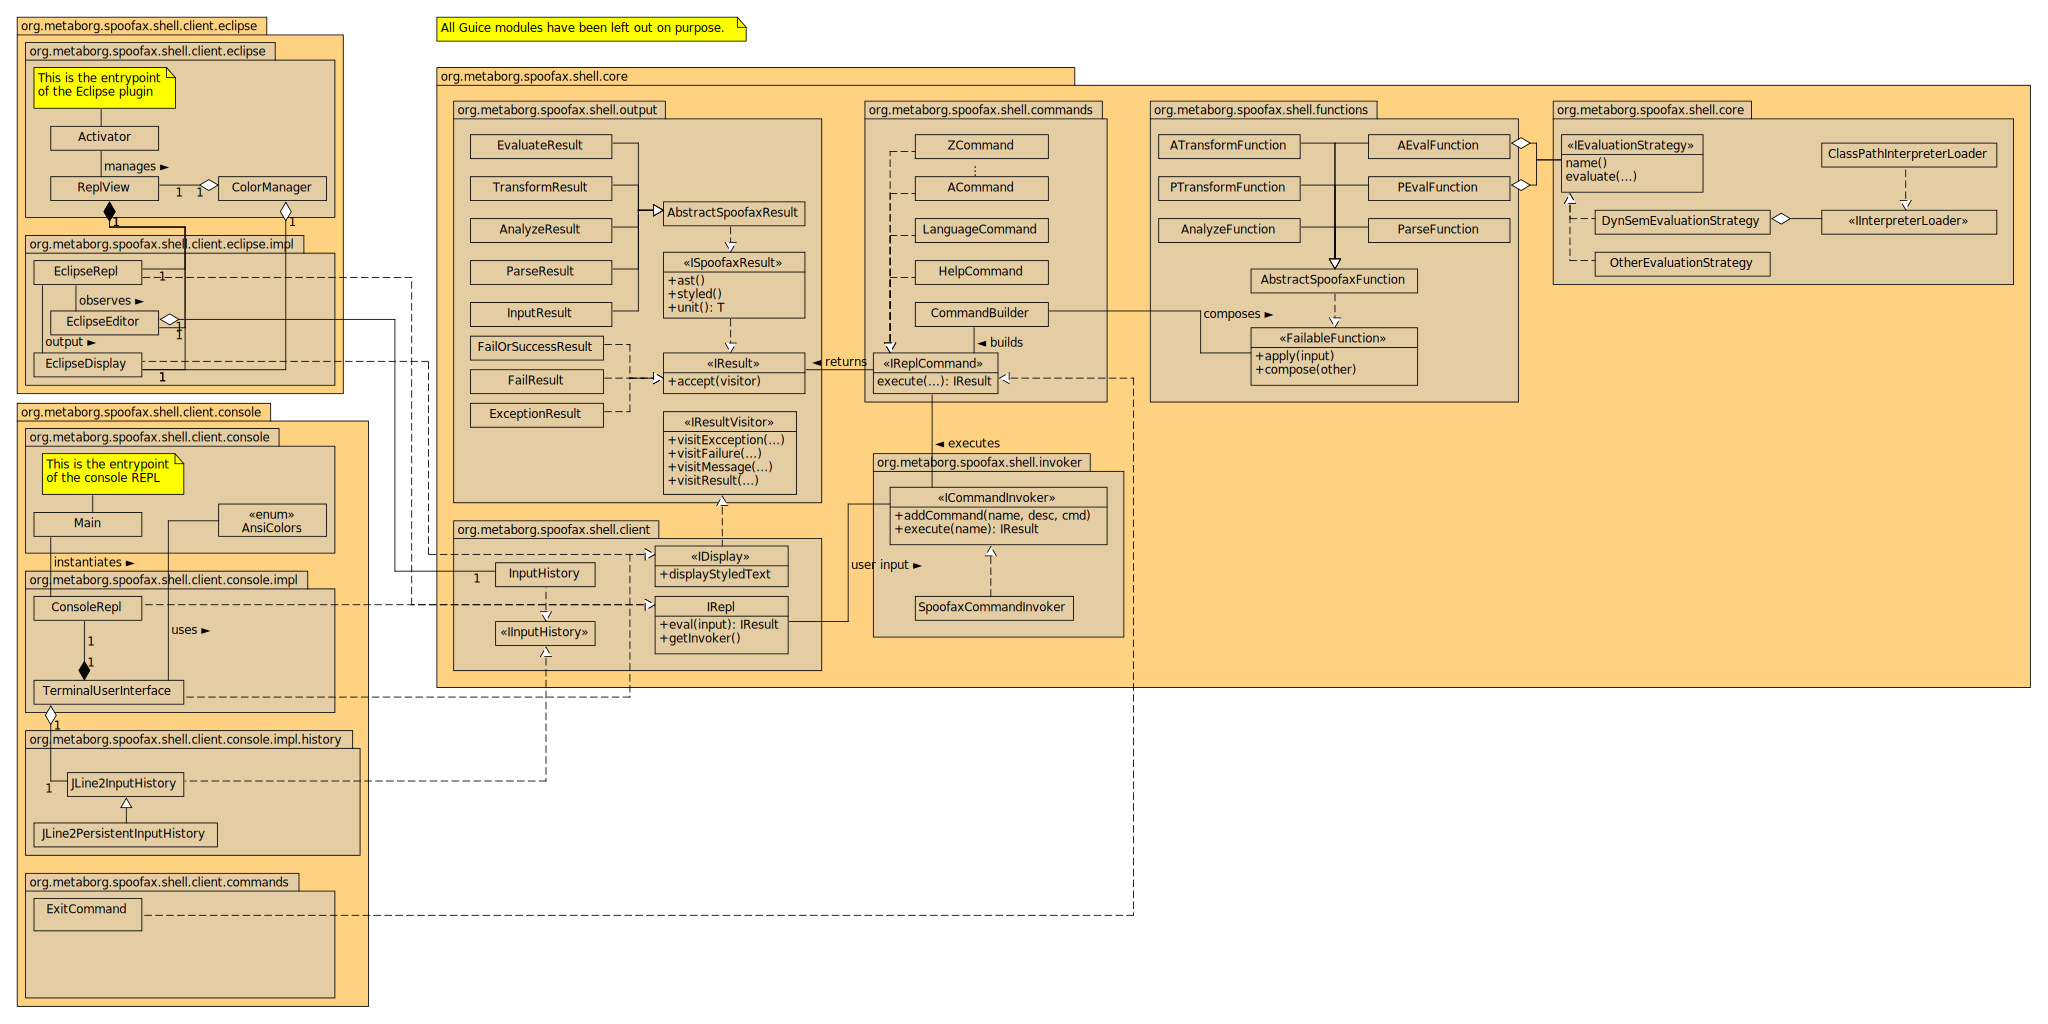
\includegraphics[angle=90,height=\textheight]{img/uml-design}
  \caption{Complete UML Diagram of the final product.}
  \label{fig:uml-design}
\end{figure}


%% Comment out for glossaries
%\glossarystyle{altlistgroup}
%\printglossaries{}

\end{document}

%%% Local Variables:
%%% mode: latex
%%% TeX-master: t
%%% End:
